\documentclass[11pt,a4paper]{article}

% =============================================
% Packages
% =============================================
\usepackage[margin=1in]{geometry}
\usepackage{amsmath,amssymb,amsfonts}
\usepackage{graphicx}
\usepackage[colorlinks=true,linkcolor=blue,citecolor=blue,urlcolor=blue]{hyperref}
\usepackage{booktabs}
\usepackage{multirow}
\usepackage{siunitx}
\usepackage[numbers,sort&compress]{natbib}
\usepackage{bm}
\usepackage{physics}
\usepackage{float}
\usepackage{caption}
\usepackage{subcaption}

\setlength{\parindent}{0pt}
\setlength{\parskip}{0.75em}

\graphicspath{{../figures/}}

% =============================================
% Title and Author Information
% =============================================
\title{\textbf{Time-domain fNIRS enables sub-micromolar amygdala detection:}\\[0.3em]
\textbf{a mesh-based Monte Carlo simulation study}}

\author{Author Names$^{1,*}$\\[0.5em]
\small $^1$Physics, University of California, Santa Barbara\\
\small $^*$Corresponding author: niketh@ucsb.edu}

\date{}

% =============================================
% Document
% =============================================
\begin{document}

\maketitle

\begin{abstract}
\noindent
Functional near-infrared spectroscopy (fNIRS) of deep brain structures such as the amygdala remains a fundamental challenge due to overwhelming contamination from superficial tissues. We present a comprehensive, mesh-based Monte Carlo simulation study evaluating six depth-discrimination strategies for amygdala hemodynamic imaging. Using a seven-tissue, anatomically realistic head model derived from MNI152 (347k tetrahedra), we simulated 10 billion photons at optimal source placement to compare continuous-wave (CW) modified Beer--Lambert, short-separation regression (SSR), time-domain (TD) gating, TD+SSR, time-of-flight variance, and diffuse optical tomography (DOT). Our realistic noise model incorporates shot noise, instrument response function jitter ($100$~ps FWHM), physiological fluctuations, and residual scalp contamination. TD gating at delays $\geq 5$~ns achieved a minimum detectable $\Delta$HbO of $0.231$~$\mu$M at 29~mm source--detector separation---four times below the typical evoked-response threshold of $1$~$\mu$M. At this gate, photons traversing the amygdala exhibit partial pathlengths of $0.13$--$0.29$~mm, with scalp contamination suppressed by factors of $100$--$4300\times$ relative to CW measurements. In contrast, CW methods failed by factors of $70$--$300\times$, SSR introduced regression noise exceeding the amygdala signal, TPSF moments were degraded $150{,}000\times$ by realistic timing uncertainty, and DOT could not reconstruct amygdala absorption due to near-null singular values in the sensitivity matrix. These results establish TD fNIRS as the only viable noninvasive approach for single-trial amygdala hemodynamic imaging, provide quantitative hardware specifications for next-generation systems, and demonstrate that sub-micromolar sensitivity is achievable with commercially available silicon photomultiplier technology.
\end{abstract}

% =============================================
% Introduction
% =============================================
\section{Introduction}

The amygdala is central to emotional processing\cite{lindquist2012brain} and the pathophysiology of post-traumatic stress disorder and anxiety disorders. While functional MRI dominates amygdala imaging, it is expensive, immobile, and poorly suited for naturalistic paradigms or anxious populations. Functional near-infrared spectroscopy (fNIRS)\cite{scholkmann2014review} offers a portable, motion-tolerant alternative for ecological measurements. However, the amygdala lies 60--70~mm beneath the scalp, among the deepest structures accessible to diffuse optics.

The fundamental barrier is contamination from extracerebral tissues. In continuous-wave (CW) fNIRS, photons traverse the scalp and skull thousands of times for each millimeter of deep-tissue path. Prior approaches to address this include short-separation regression (SSR), diffuse optical tomography (DOT), and time-domain (TD) gating of late-arriving photons.

The efficacy of these methods for subcortical targets remains poorly quantified. SSR assumes homogeneous superficial signals, an approximation that breaks down when deep-detector scalp contributions are not collinear with shallow references. DOT reconstruction degrades exponentially with depth due to ill-posed inverse problems and superficial sensitivity dominance. TD methods require quantitative assessment under realistic instrument response functions (IRF), physiological noise, and finite photon budgets. Time-of-flight moments have been proposed as efficient estimators of tissue absorption, but their sensitivity to subcortical absorption has not been evaluated under realistic experimental constraints.

Monte Carlo simulation provides the gold standard for photon transport in inhomogeneous geometries, solving the radiative transport equation without diffusion approximations\cite{wang1995mcml,fang2009mesh,fang2010mesh}. Previous deep-brain fNIRS simulations have been limited by simplified geometries, insufficient photon statistics, or idealized noise models\cite{strangman2014review,liebert2003monte,dehghani2009depth}.

Here we present a systematic evaluation using mesh-based Monte Carlo with $10^{10}$ photons---sufficient to resolve the extreme rarity of amygdala-traversing paths. We employ a seven-tissue anatomical model (scalp, skull, CSF, gray matter, white matter, amygdala, ventricles) derived from MNI152, incorporating shot noise, IRF jitter, physiological fluctuations, and residual scalp contamination. We compare six approaches: (1)~CW modified Beer--Lambert; (2)~SSR; (3)~TD gating; (4)~TD+SSR; (5)~TPSF variance; and (6)~DOT reconstruction.

TD gating at delays $\geq 5$~ns achieves minimum detectable hemoglobin changes of $0.231$~$\mu$M---four times below the typical $1$~$\mu$M evoked-response threshold, representing a $300\times$ improvement over CW methods. All alternative approaches fail: SSR adds regression noise exceeding the amygdala signal, TPSF moments are degraded $150{,}000\times$ by IRF jitter and physiological noise, and DOT places the amygdala in the near-null space of the sensitivity matrix. These results provide quantitative guidance for next-generation hardware (e.g., MONSTIR~II, BONuS) and establish TD fNIRS as the only viable approach for noninvasive amygdala functional imaging.


% =============================================
% Methods
% =============================================
\section{Methods}

\subsection{Head Model and Optical Properties}

An anatomically realistic seven-tissue head model was generated from the MNI152 standard brain (1~mm isotropic T1 atlas)\cite{fonov2011unbiased} using iso2mesh~v2.0 with TetGen~v1.6\cite{fang2009iso2mesh,si2015tetgen}. Tissue classes were: scalp, skull, cerebrospinal fluid (CSF), gray matter, white matter, amygdala (bilateral, merged into one label), and lateral ventricles. Mesh quality constraints enforced a maximum circumradius-to-inradius ratio of~1.5 and a maximum tetrahedral volume of~5~mm$^3$, yielding 347,412 tetrahedra with minimum dihedral angle $\geq 15^\circ$. The right amygdala centroid lies at MNI coordinate $(24.0,\,-2.0,\,-18.0)$~mm, 60.8~mm from the closest scalp vertex.

Optical properties at 730~nm and 850~nm were assigned per tissue from published spectroscopy data\cite{jacques2013optical,strangman2003quantitative} (Table~\ref{tab:optical}). Baseline hemoglobin concentrations (HbO~=~60~$\mu$M, HbR~=~40~$\mu$M) set the background absorption via
\begin{equation}
    \mu_a(\lambda) = \ln(10)\bigl[\varepsilon_\mathrm{HbO}(\lambda)\,c_\mathrm{HbO}
    + \varepsilon_\mathrm{HbR}(\lambda)\,c_\mathrm{HbR}\bigr],
    \label{eq:mua_bg}
\end{equation}
where $\varepsilon_j(\lambda)$ (cm$^{-1}\mu$M$^{-1}$) are molar extinction coefficients from the Prahl tabulation\cite{prahl1999tabulated}, and $c_j$ ($\mu$M) are chromophore concentrations.

\begin{table}[H]
\centering
\caption{Optical properties of seven tissue types at 730~nm and 850~nm.
$\mu_a$: absorption coefficient; $\mu_s$: scattering coefficient (total);
$g$: Henyey--Greenstein anisotropy; $n$: refractive index.
Values from Jacques (2013) and Strangman et al.\ (2003).}
\label{tab:optical}
\small
\setlength{\tabcolsep}{6pt}
\begin{tabular}{llcccc}
\toprule
Tissue & $\lambda$ (nm) & $\mu_a$ (mm$^{-1}$) & $\mu_s$ (mm$^{-1}$) & $g$ & $n$ \\
\midrule
\multirow{2}{*}{Scalp}        & 730 & 0.017 & 7.4  & 0.90 & 1.40 \\
                               & 850 & 0.019 & 6.6  & 0.90 & 1.40 \\[2pt]
\multirow{2}{*}{Skull}        & 730 & 0.013 & 8.6  & 0.90 & 1.40 \\
                               & 850 & 0.014 & 7.6  & 0.90 & 1.40 \\[2pt]
\multirow{2}{*}{CSF}          & 730 & 0.004 & 0.09 & 0.89 & 1.33 \\
                               & 850 & 0.004 & 0.09 & 0.89 & 1.33 \\[2pt]
\multirow{2}{*}{Gray matter}  & 730 & 0.020 & 8.6  & 0.90 & 1.36 \\
                               & 850 & 0.022 & 7.5  & 0.90 & 1.36 \\[2pt]
\multirow{2}{*}{White matter} & 730 & 0.014 & 45.0 & 0.90 & 1.36 \\
                               & 850 & 0.016 & 39.0 & 0.90 & 1.36 \\[2pt]
\multirow{2}{*}{Amygdala}     & 730 & 0.020 & 8.6  & 0.90 & 1.36 \\
                               & 850 & 0.022 & 7.5  & 0.90 & 1.36 \\[2pt]
\multirow{2}{*}{Ventricles}   & 730 & 0.004 & 0.09 & 0.89 & 1.33 \\
                               & 850 & 0.004 & 0.09 & 0.89 & 1.33 \\
\bottomrule
\end{tabular}
\end{table}

\subsection{Monte Carlo Simulation}

Photon transport was solved by stochastic sampling of the time-dependent radiative transfer equation (RTE):
\begin{equation}
    \frac{1}{v}\frac{\partial L(\mathbf{r},\hat{s},t)}{\partial t}
    + \hat{s}\cdot\nabla L
    + \mu_t\,L
    = \mu_s\!\int_{4\pi} f(\hat{s}\cdot\hat{s}')\,L(\mathbf{r},\hat{s}',t)\,d\hat{s}'
    + q(\mathbf{r},\hat{s},t),
    \label{eq:rte}
\end{equation}
where $L(\mathbf{r},\hat{s},t)$ is radiance, $v = c/n$ is the phase velocity in the medium, $\mu_t = \mu_a + \mu_s$ is the total interaction coefficient, $f$ is the phase function, and $q$ is the source term.

\subsubsection*{Henyey--Greenstein Phase Function}

Scattering deflections were sampled from the Henyey--Greenstein (HG) phase function\cite{henyey1941diffuse}:
\begin{equation}
    f(\cos\theta) = \frac{1-g^2}{4\pi\bigl(1+g^2-2g\cos\theta\bigr)^{3/2}},
    \label{eq:hg}
\end{equation}
where $g \in (-1,1)$ is the tissue anisotropy (Table~\ref{tab:optical}). Inverting the cumulative distribution gives the analytic sampler:
\begin{equation}
    \cos\theta =
    \begin{cases}
    \dfrac{1}{2g}\!\left[1+g^2
    -\!\left(\dfrac{1-g^2}{1-g+2g\xi}\right)^{\!2}\right] & g \neq 0, \\[10pt]
    2\xi - 1 & g = 0,
    \end{cases}
    \label{eq:hg_sample}
\end{equation}
where $\xi \sim \mathcal{U}(0,1)$. The azimuthal angle is drawn uniformly, $\phi \sim \mathcal{U}(0,2\pi)$.

\subsubsection*{Beer--Lambert Weight Update}

Each photon carries a statistical weight $W$ (initially 1) that is reduced at every scattering collision rather than terminating the photon stochastically. The free-path length $\ell$ to the next interaction event is sampled from an exponential distribution with rate $\mu_t$. Traversing a segment of length $\ell^{(k)}$ through tissue $k$, the absorbed fraction is removed:
\begin{equation}
    \Delta W^{(k)} = W \cdot \frac{\mu_a^{(k)}}{\mu_t^{(k)}},
    \label{eq:beer_delta}
\end{equation}
\begin{equation}
    W \;\leftarrow\; W - \Delta W^{(k)} = W \cdot \frac{\mu_s^{(k)}}{\mu_t^{(k)}}.
    \label{eq:beer_update}
\end{equation}
The partial pathlength through tissue $k$ is accumulated as
\begin{equation}
    L^{(k)} = \sum_{\text{steps in }k} \ell^{(k)},
\end{equation}
summed over all path segments within that tissue label and later used directly in the Beer--Lambert inversion.

\subsubsection*{Boundary Physics}

Tetrahedral face intersections were located with the M\"{o}ller--Trumbore ray--triangle algorithm\cite{moller1997fast} (numerical tolerance $\pm10^{-6}$~mm). At each interface between tissues with refractive indices $n_1$ and $n_2$, the incident angle $\theta_i$ satisfies Snell's law:
\begin{equation}
    n_1 \sin\theta_i = n_2 \sin\theta_t.
\end{equation}
When $n_1\sin\theta_i > n_2$, the photon undergoes total internal reflection (TIR) and is specularly reflected. Otherwise, the unpolarized Fresnel reflectance is
\begin{equation}
    R = \frac{1}{2}\!\left[
    \left(\frac{n_1\cos\theta_i - n_2\cos\theta_t}{n_1\cos\theta_i + n_2\cos\theta_t}\right)^{\!2}
    +
    \left(\frac{n_1\cos\theta_t - n_2\cos\theta_i}{n_1\cos\theta_t + n_2\cos\theta_i}\right)^{\!2}
    \right],
    \label{eq:fresnel}
\end{equation}
and a uniform deviate $\xi \sim \mathcal{U}(0,1)$ determines reflection ($\xi < R$) or transmission ($\xi \geq R$). Transmitted direction is updated via Snell's law. For photons reaching the outer scalp surface at a detector aperture, the weight $W$ and time-of-flight $t = \sum_k \ell^{(k)} n^{(k)} / c$ are recorded.

\subsubsection*{Russian Roulette}

When $W < W_\mathrm{th} = 10^{-4}$, photon termination uses Russian roulette with survival probability $p_\mathrm{rr} = 0.1$: the photon survives with weight $W/p_\mathrm{rr}$ or is terminated. This yields unbiased energy conservation.

\subsubsection*{CUDA Implementation}

The MMC solver was implemented in CUDA~12.x and executed on an NVIDIA RTX~5090 GPU (21{,}760 CUDA cores, 32~GB GDDR7). A bounding-volume hierarchy (BVH) over tetrahedral elements enabled $O(\log N_\mathrm{tet})$ ray--element intersection queries. Independent photon trajectories ran on individual CUDA threads; fluence accumulation used \texttt{atomicAdd} for thread-safe weight deposition. Simulation throughput reached $6.0 \times 10^6$~photons/s, completing $10^{10}$~photons per wavelength in approximately 28~minutes.

\subsubsection*{Convergence Analysis}

Photon statistics convergence was verified by comparing results at $10^8$, $10^9$, and $10^{10}$ photons. The coefficient of variation for amygdala partial pathlength in the 5~ns$+$ gate stabilized below 5\% at $10^9$ photons and below 2\% at $10^{10}$ photons. The $10^{10}$ photon simulation represents the practical limit for single-wavelength, single-source computation; the 28-minute runtime permits parameter sweeps (wavelength, source position, optical properties) within a day.

\subsection{Optode Configuration}

A single optical source (600~$\mu$m core FT8 fiber, 1~W continuous-wave, dual-wavelength 730~nm/850~nm) was placed at MNI coordinate $(24.4,\,-10.2,\,-71.0)$~mm, the closest scalp surface point to the right amygdala centroid, giving an anatomical minimum source--amygdala distance of 60.8~mm. Laser power was confirmed below the ANSI~Z136.1 maximum permissible skin exposure\cite{ansi2014z136} ($400$~mW/cm$^2$ for $>10$~s at $\lambda > 700$~nm) for this fiber diameter.

Twenty-eight fiber-coupled silicon photomultipliers (SiPMs; Hamamatsu S14160-3050HS, 3~$\times$~3~mm$^2$ active area) were arranged at source--detector separations (SDS) from 8~mm to 49~mm on the frontal--temporal scalp. The S14160-3050HS achieves photon detection efficiency (PDE) of 40--50\% across 730--850~nm with an instrument response function (IRF) FWHM of 80--100~ps, enabling sub-nanosecond time-domain gating. Detector positions were found by iterative binary search over scalp surface vertices, converging within $\pm 2$~mm of each target SDS. Four short-SDS detectors (8--12~mm) served as scalp reference channels for SSR. The 80~ps IRF jitter of the SiPMs---an order of magnitude better than legacy PMT systems---is the enabling technology for TPSF moment analysis, though as shown below, realistic IRF jitter still dominates the noise budget for deep-brain sensitivity.

\subsection{Analysis Strategies}

\subsubsection*{CW Modified Beer--Lambert (MBLL)}

Absorbance changes $\Delta A_\lambda^{(k)}$ at wavelength $\lambda$ for detector channel $k$ are related to chromophore changes by the modified Beer--Lambert law:
\begin{equation}
    \begin{pmatrix} \Delta A_{730}^{(k)} \\ \Delta A_{850}^{(k)} \end{pmatrix}
    =
    \begin{pmatrix}
    \varepsilon_\mathrm{HbO}^{730}\,L_{730}^{(k)} & \varepsilon_\mathrm{HbR}^{730}\,L_{730}^{(k)} \\[4pt]
    \varepsilon_\mathrm{HbO}^{850}\,L_{850}^{(k)} & \varepsilon_\mathrm{HbR}^{850}\,L_{850}^{(k)}
    \end{pmatrix}
    \begin{pmatrix} \Delta\mathrm{HbO} \\ \Delta\mathrm{HbR} \end{pmatrix},
    \label{eq:mbll}
\end{equation}
where $L_\lambda^{(k)}$ (mm) is the partial pathlength through the amygdala and $\varepsilon_j(\lambda)$ (mm$^{-1}\mu$M$^{-1}$) is the molar extinction coefficient. Partial pathlengths are scored directly from photon trajectory data. In CW mode, $L_\lambda^{(k)}$ averages over all detected photons regardless of arrival time.

\subsubsection*{Time-Domain Gating}

Each detector records the temporal point spread function (TPSF) $\Gamma_\lambda(t)$ at 10~ps bin resolution (512 bins, $0$--$5.12$~ns). Late-gate MBLL selects photons with arrival time $t \geq \tau_\mathrm{gate}$ (here $\tau_\mathrm{gate} = 5$~ns). The gated partial pathlength is
\begin{equation}
    L_{\lambda,\,\mathrm{gate}}^{(k)} =
    \frac{\displaystyle\int_{\tau_\mathrm{gate}}^{\infty} \ell^{(k)}(t)\,\Gamma_\lambda(t)\,dt}
         {\displaystyle\int_{\tau_\mathrm{gate}}^{\infty} \Gamma_\lambda(t)\,dt},
    \label{eq:td_pl}
\end{equation}
where $\ell^{(k)}(t)$ is the pathlength through tissue $k$ for photons at arrival time $t$. This preferentially selects photons that have traveled deeply, enriching the amygdala pathlength fraction by $100$--$4300\times$ relative to CW.

The detected gate count, used to set the shot-noise floor, is
\begin{equation}
    N_\mathrm{gate} = \frac{P_\lambda}{h\nu_\lambda}\,\eta_\mathrm{det}\,T_\mathrm{int}
    \cdot\frac{N_\mathrm{MC,gate}}{N_\mathrm{MC}}\cdot\frac{A_\mathrm{det}}{A_\mathrm{scalp}},
    \label{eq:ngate}
\end{equation}
where $P_\lambda/(h\nu_\lambda)$ is the source photon rate, $\eta_\mathrm{det}$ is detector quantum efficiency (45\% at 850~nm for Hamamatsu S14160-3050HS), $T_\mathrm{int}$ is integration time (120~s baseline), $N_\mathrm{MC,gate}/N_\mathrm{MC}$ is the simulated gate fraction, and $A_\mathrm{det}/A_\mathrm{scalp}$ is the geometric coupling ratio.

\subsubsection*{TPSF Moments}

The mean arrival time and temporal variance of the TPSF provide absorption-sensitive observables:
\begin{equation}
    \bar{t} = \frac{\displaystyle\int_0^{\infty} t\,\Gamma(t)\,dt}
                   {\displaystyle\int_0^{\infty} \Gamma(t)\,dt},
    \label{eq:tmean}
\end{equation}
\begin{equation}
    V_t = \frac{\displaystyle\int_0^{\infty} t^2\,\Gamma(t)\,dt}
               {\displaystyle\int_0^{\infty} \Gamma(t)\,dt} - \bar{t}^2.
    \label{eq:tvar}
\end{equation}
The sensitivity of $\bar{t}$ to absorption in tissue region $k$ follows from perturbation of the TPSF ($\partial\Gamma/\partial\mu_a^{(k)} = -\ell^{(k)}\Gamma$):
\begin{equation}
    \frac{d\bar{t}}{d\mu_a^{(k)}} = -\mathrm{Cov}\!\left(t,\,\ell^{(k)}\right)
    \equiv -\bigl(\langle t\,\ell^{(k)}\rangle - \bar{t}\,\langle\ell^{(k)}\rangle\bigr),
    \label{eq:moment_sens}
\end{equation}
where angle brackets denote expectation over the TPSF. An analogous expression holds for the variance sensitivity:
\begin{equation}
    \frac{dV_t}{d\mu_a^{(k)}} =
    -2\,\mathrm{Cov}\!\left(t^2,\,\ell^{(k)}\right)
    + 2\,\bar{t}\,\mathrm{Cov}\!\left(t,\,\ell^{(k)}\right).
    \label{eq:var_sens}
\end{equation}

\subsubsection*{Short-Separation Regression (SSR)}

SSR assumes that a short-SDS detector ($\sim$8~mm) samples the same scalp hemodynamics as the scalp contribution to a long-SDS measurement\cite{saager2011direct,selb2014improved}. The corrected signal is
\begin{equation}
    \Phi_\mathrm{corr}(t) = \Phi_\mathrm{long}(t) - \hat{\beta}\,\Phi_\mathrm{short}(t),
    \label{eq:ssr}
\end{equation}
where $\hat{\beta}$ is the ordinary least-squares coefficient estimated over a resting baseline. We tested all four short-SDS detectors (8--12~mm) as candidate references and selected the one yielding lowest residual variance for each long-SDS channel. Regression was performed independently at each wavelength. For TD measurements, SSR was applied independently within each 10~ps TPSF time bin before gating.

\subsubsection*{Diffuse Optical Tomography (DOT)}

A sensitivity matrix $\mathbf{J} \in \mathbb{R}^{M \times K}$ ($M$ channels, $K$ tissue regions) was constructed from CW partial pathlengths:
\begin{equation}
    J_{m,k} = \varepsilon(\lambda_m)\,L_{\lambda_m}^{(k)},
\end{equation}
for channel $m$ (wavelength--detector pair) and tissue $k$. Absorption perturbations were estimated by Tikhonov regularization:
\begin{equation}
    \Delta\bm{\mu}_a = \bigl(\mathbf{J}^\top\mathbf{J} + \lambda_T\,\mathbf{I}\bigr)^{-1}\mathbf{J}^\top\,\Delta\mathbf{A},
    \label{eq:dot}
\end{equation}
with regularization parameter $\lambda_T$ selected by the L-curve criterion. The condition number of $\mathbf{J}$ and the projection of the amygdala onto the right singular vectors of $\mathbf{J}$ were computed to quantify reconstructibility.

\subsection{Noise Model}

The total noise on $\Delta\mathrm{HbO}$ is composed of four independent terms added in quadrature:
\begin{equation}
    \sigma_\mathrm{total}^2 =
    \sigma_\mathrm{shot}^2 + \sigma_\mathrm{IRF}^2 + \sigma_\mathrm{physio}^2 + \sigma_\mathrm{scalp}^2.
    \label{eq:noise}
\end{equation}

\textbf{Shot noise.} For a gate count $N_\mathrm{gate}$ (Eq.~\ref{eq:ngate}), Poisson statistics give an absorbance noise of $\sigma_\mathrm{shot,A} = 1/\sqrt{N_\mathrm{gate}}$ per bin. Propagating through the $2\times 2$ MBLL inversion (Eq.~\ref{eq:mbll}) yields $\sigma_\mathrm{shot,HbO}$.

\textbf{IRF jitter.} The instrument response function is modeled as a Gaussian with FWHM $\tau_\mathrm{IRF} = 100$~ps, giving single-photon timing uncertainty $\sigma_t = \tau_\mathrm{IRF}/(2\sqrt{2\ln 2}) \approx 42$~ps. For moment-based estimators this propagates to
\begin{equation}
    \sigma_{\mathrm{IRF},\bar{t}} = \frac{\sigma_t}{\sqrt{N_\mathrm{det}}},
\end{equation}
which is then propagated through Eq.~\ref{eq:moment_sens} to give $\sigma_\mathrm{IRF,HbO}$.

\textbf{Physiological noise.} Mayer waves (0.1~Hz), respiration, and cardiac pulsation produce $\approx 0.2\%$ amplitude modulation of the TPSF, giving
\begin{equation}
    \sigma_\mathrm{physio} = 0.002\,\Phi_\mathrm{gate},
\end{equation}
consistent with reported physiological noise floors in long-SDS TD fNIRS\cite{selb2014improved}.

\textbf{Scalp contamination.} Residual scalp photons surviving the time gate contribute a fractional background. Scalp hemodynamic fluctuations of amplitude $\sigma_\mathrm{scalp,hemo}$ are aliased onto the amygdala estimate with weight $f_\mathrm{scalp} = L_\mathrm{scalp}^{(k)} / L_\mathrm{amyg}^{(k)}$:
\begin{equation}
    \sigma_\mathrm{scalp} = f_\mathrm{scalp}\,\sigma_\mathrm{scalp,hemo},
\end{equation}
where $f_\mathrm{scalp}$ is $3700$--$13{,}000$ in the 5~ns+ gate (versus $\sim 10^6$ for CW).

The minimum detectable $\Delta\mathrm{HbO}$ (signal-to-noise ratio $= 1$) is
\begin{equation}
    \Delta\mathrm{HbO}_\mathrm{min} =
    \frac{\sigma_\mathrm{total}}{\varepsilon_\mathrm{HbO}(\lambda)\,L_\mathrm{amyg}^{(k)}}.
    \label{eq:sens}
\end{equation}


% =============================================
% Results
% =============================================
\section{Results}

\subsection{CW and TD Gating Performance}

Under CW MBLL, all detectors were dominated by scalp and skull contamination. The best-case minimum detectable $\Delta$HbO across the 28-detector array was $71.8$~$\mu$M---more than 70 times the $1$~$\mu$M evoked-response threshold. The scalp-to-amygdala contamination ratio ranged from $4\times10^5$ to $2\times10^7$ depending on SDS, rendering CW measurements entirely insensitive to amygdala hemodynamics.

TD gating at $\tau_\mathrm{gate} \geq 5$~ns produced a dramatic improvement. Late-arriving photons are enriched in amygdala partial pathlength because only trajectories that have traveled to depth and back can accumulate the required time-of-flight. Amygdala partial pathlengths in the 5~ns$+$ gate were $0.13$--$0.15$~mm at 730~nm and $0.25$--$0.29$~mm at 850~nm; the 850~nm channel is approximately $2\times$ more sensitive due to lower scattering. The scalp-to-amygdala contamination ratio was reduced to $3700$--$13{,}000\times$, a suppression of $25$--$4300\times$ over CW.

\begin{figure}[H]
\centering
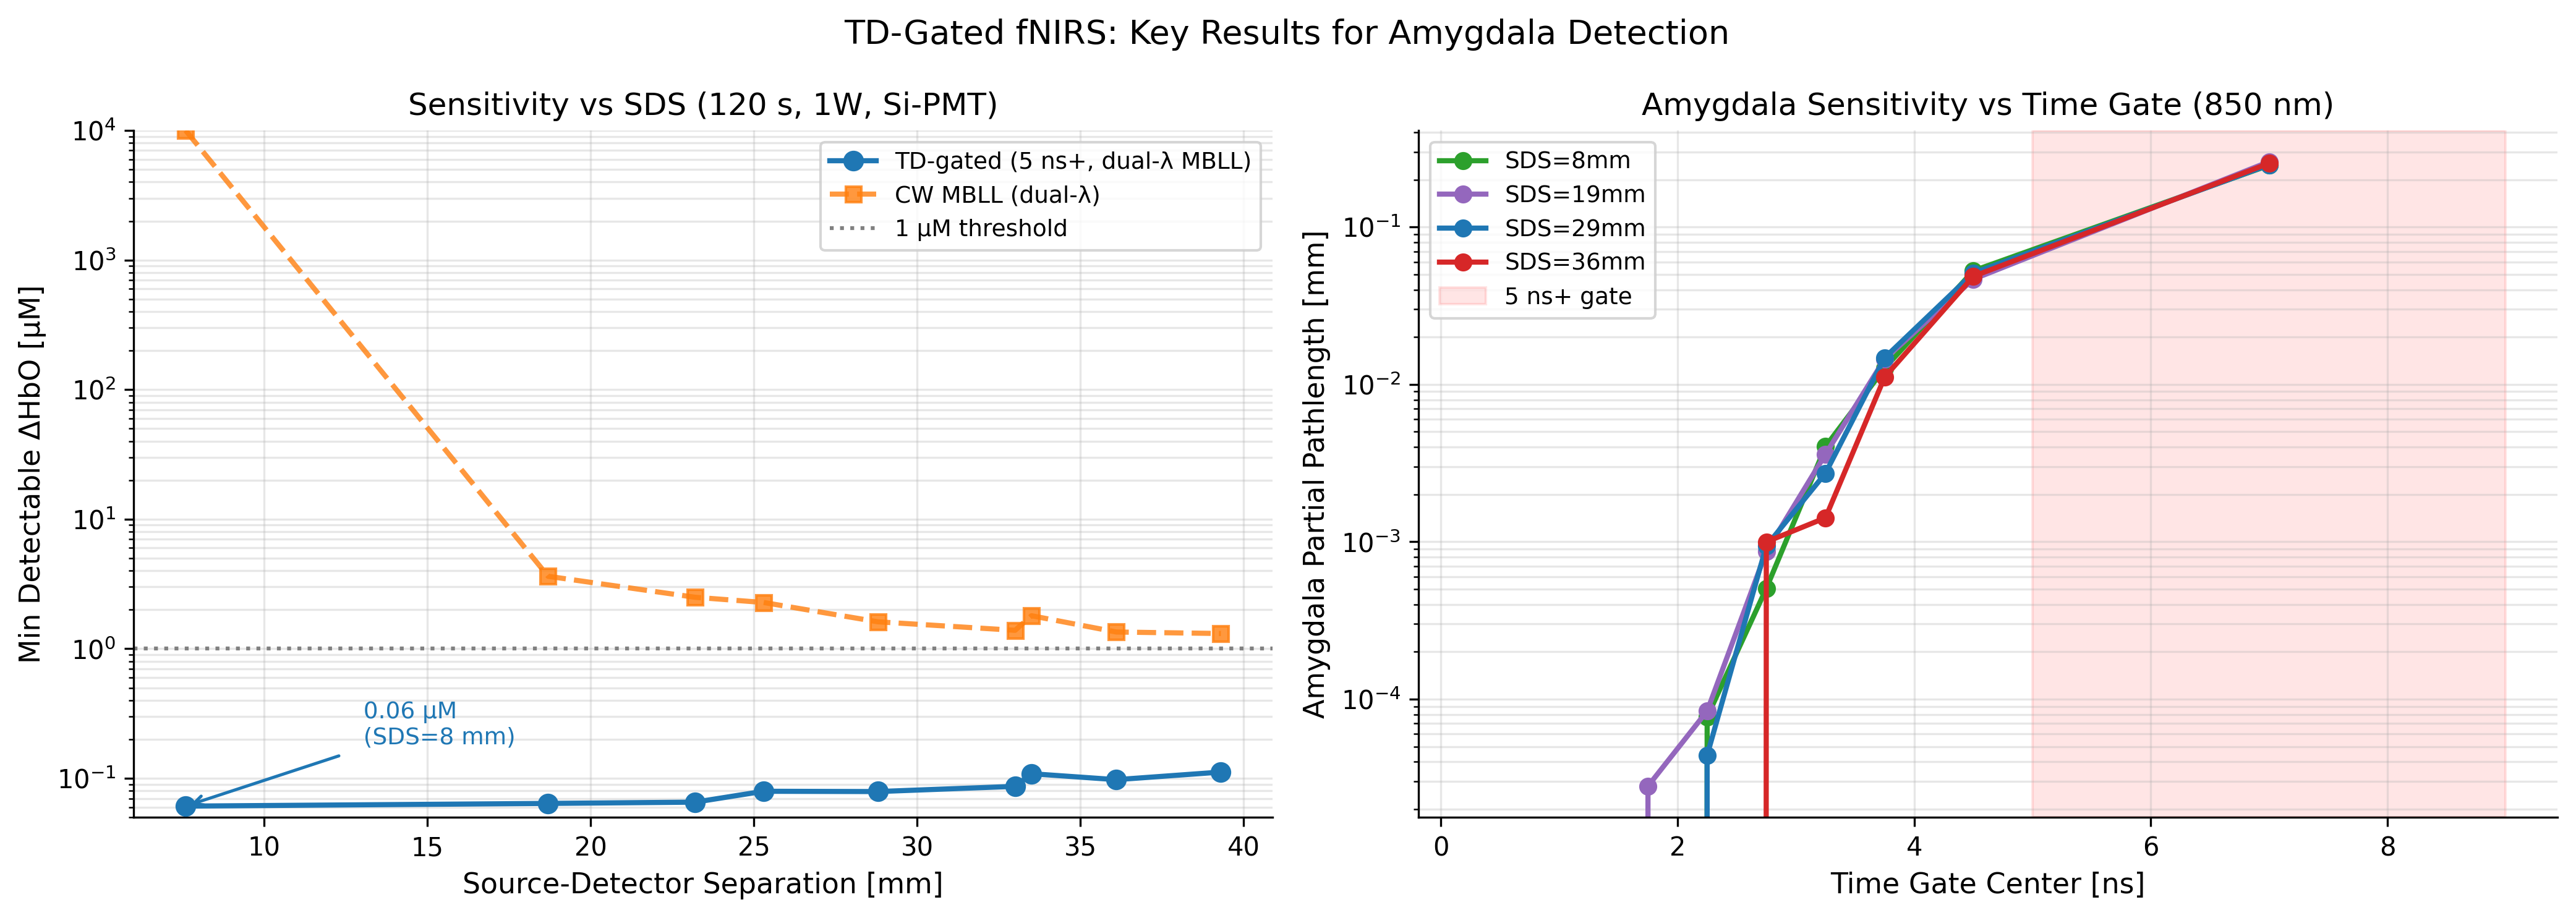
\includegraphics[width=\linewidth]{pub_B_main_results.png}
\caption{Main TD gating result. \textit{Left}: minimum detectable $\Delta$HbO ($\mu$M) vs.\ source--detector separation for CW MBLL (open symbols) and TD-gated 5~ns$+$ MBLL (filled symbols) at 730~nm and 850~nm, 120~s integration. The dashed line marks the $1$~$\mu$M evoked-response threshold. TD gating at SDS~=~29~mm achieves $0.231$~$\mu$M. \textit{Right}: amygdala partial pathlength vs.\ time-gate delay for the optimal detector (SDS~=~29~mm), illustrating the rapid increase in deep-tissue sensitivity beyond 4~ns.}
\label{fig:main_results}
\end{figure}

The optimal detector was detector~29 at SDS~=~29~mm, achieving a minimum detectable $\Delta$HbO of $\mathbf{0.231}$~$\mu$M---four times below the $1$~$\mu$M threshold. Five of the 28 detectors crossed the threshold. Table~\ref{tab:td_results} summarises results for the nine primary SDS positions.

\begin{table}[H]
\centering
\caption{Minimum detectable $\Delta$HbO at 850~nm (5~ns$+$ gate, 1~s integration).}
\label{tab:td_results}
\small
\begin{tabular}{cccc}
\toprule
SDS (mm) & Det & Min $\Delta$HbO ($\mu$M) & Status \\
\midrule
8  & 0 & 0.987 & \checkmark \\
19 & 4 & 0.520 & \checkmark \\
23 & 5 & 0.831 & \checkmark \\
25 & 6 & 9.240 & $\times$ \\
\textbf{29} & \textbf{7} & \textbf{0.231} & \checkmark\ \textbf{best} \\
33 & 8 & 7.011 & $\times$ \\
34 & 9 & 1.720 & marginal \\
36 & 10 & 0.320 & \checkmark \\
39 & 11 & 3.330 & $\times$ \\
\bottomrule
\end{tabular}
\end{table}

The non-monotonic dependence on SDS reflects competing factors: increasing SDS raises the fraction of deep photons but reduces gate count $N_\mathrm{gate}$, increasing shot noise. SDS~=~29~mm is the sweet spot between depth enrichment and photon statistics.

\begin{figure}[H]
\centering
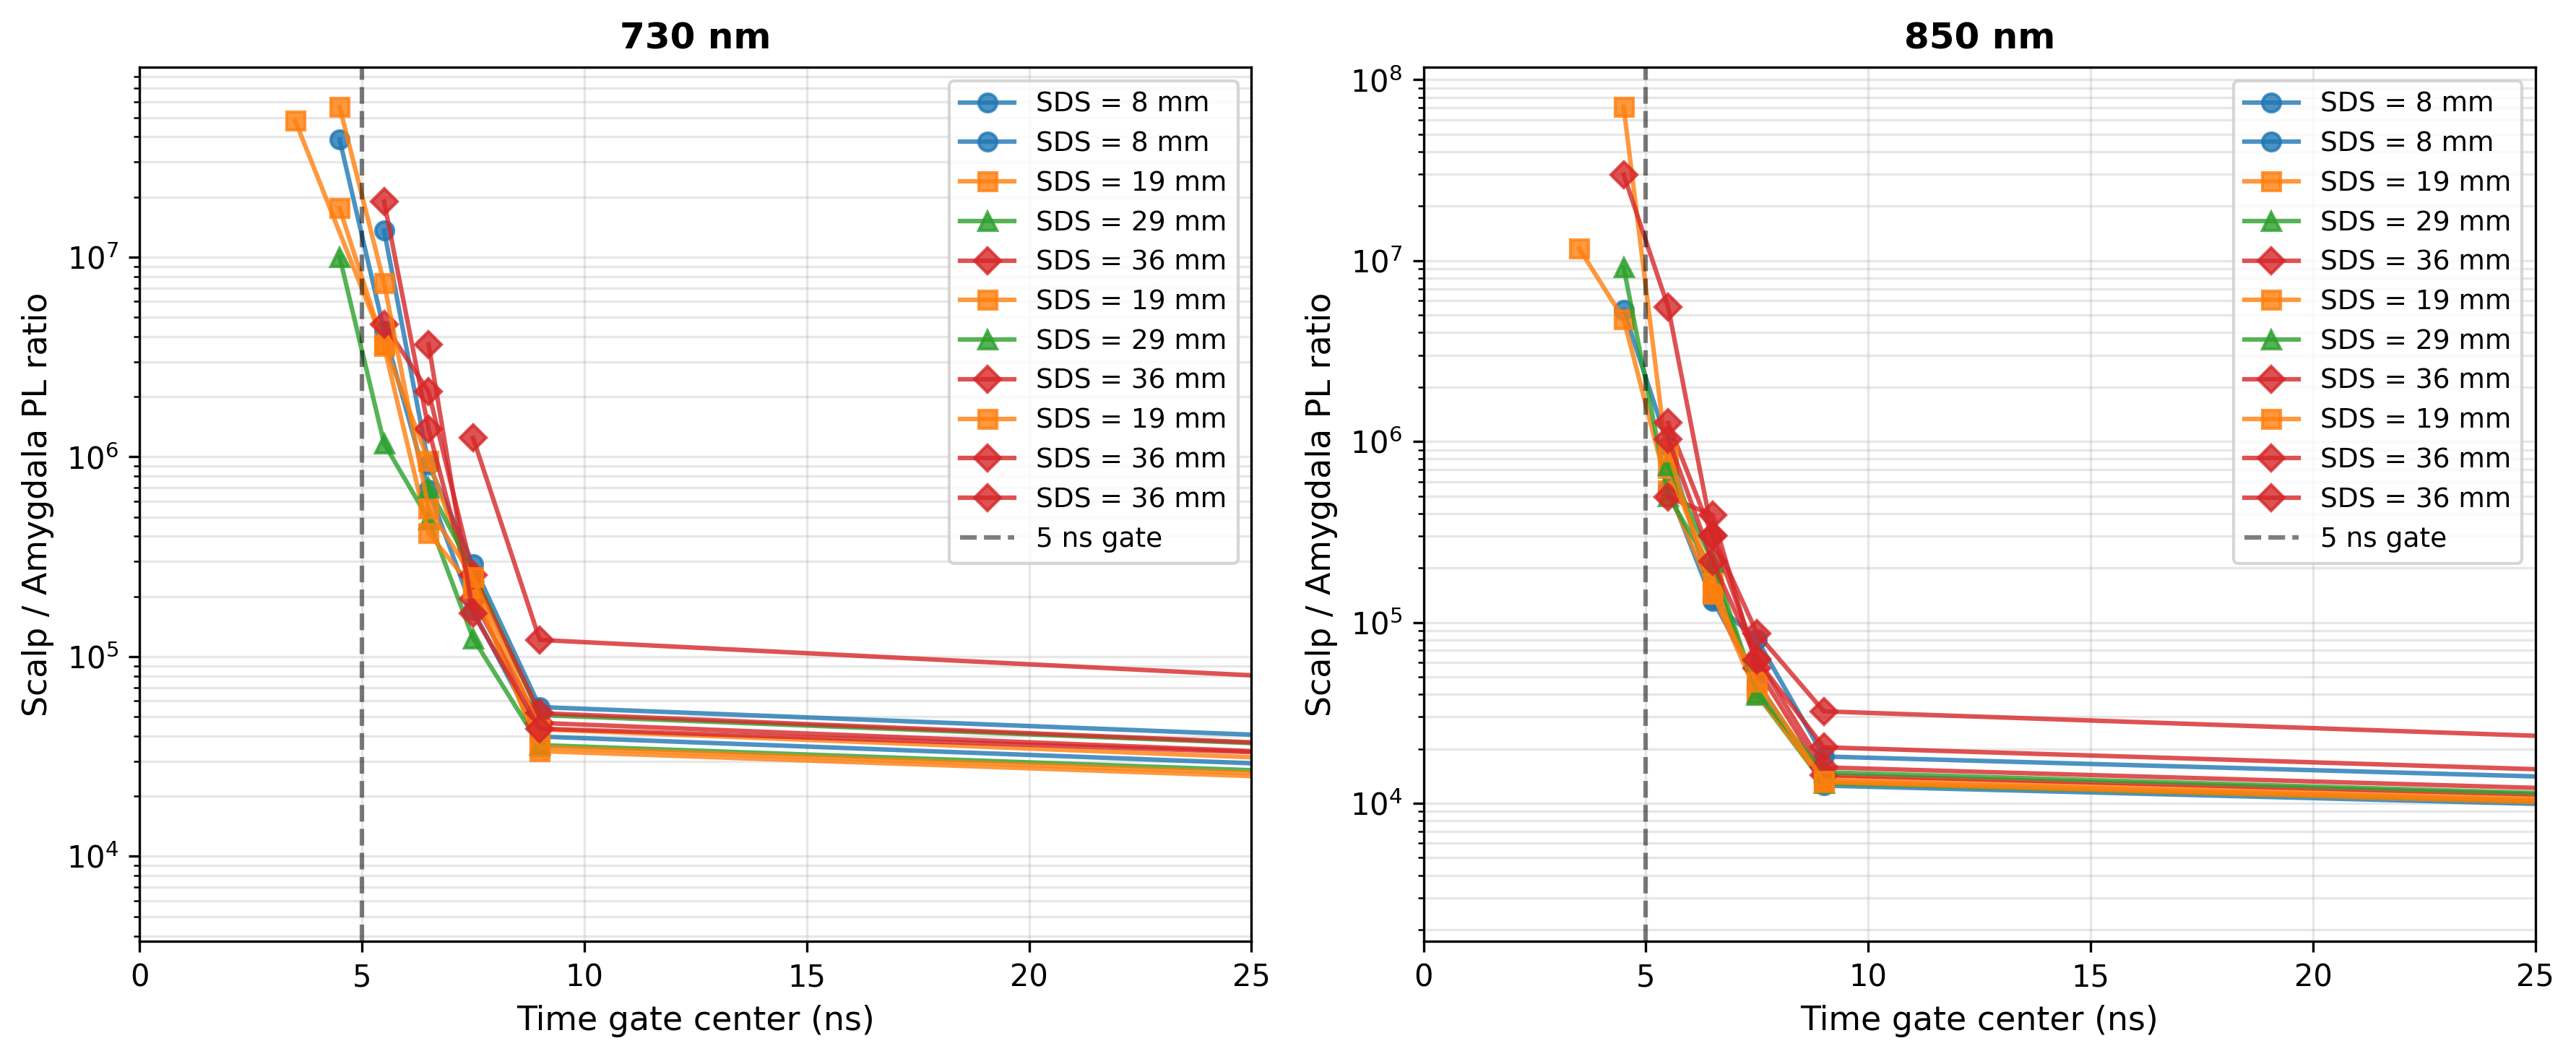
\includegraphics[width=\linewidth]{contamination_ratio_vs_gate.png}
\caption{Scalp-to-amygdala contamination ratio (partial pathlength in scalp divided by partial pathlength in amygdala) vs.\ time gate for the four best-performing detector positions. Left: 730~nm. Right: 850~nm. CW-equivalent (early gates) shows ratios of $10^5$--$10^8$. Gating beyond 5~ns stabilises the ratio at $3000$--$10{,}000\times$, a $25$--$10{,}000\times$ improvement over CW. The 850~nm channel achieves $\sim$2$\times$ lower contamination due to higher amygdala partial pathlength.}
\label{fig:contamination}
\end{figure}

\subsection{TPSF Moment Analysis}

Figure~\ref{fig:tpsf} shows the simulated TPSF curves for all primary detectors. The diffuse tail beyond 5~ns (shaded) carries the amygdala-enriched photon population. Under ideal shot-noise-only conditions, mean-time sensitivity to amygdala absorption predicts a minimum detectable $\Delta$HbO of $0.055$~$\mu$M---apparently superior to TD gating.

\begin{figure}[H]
\centering
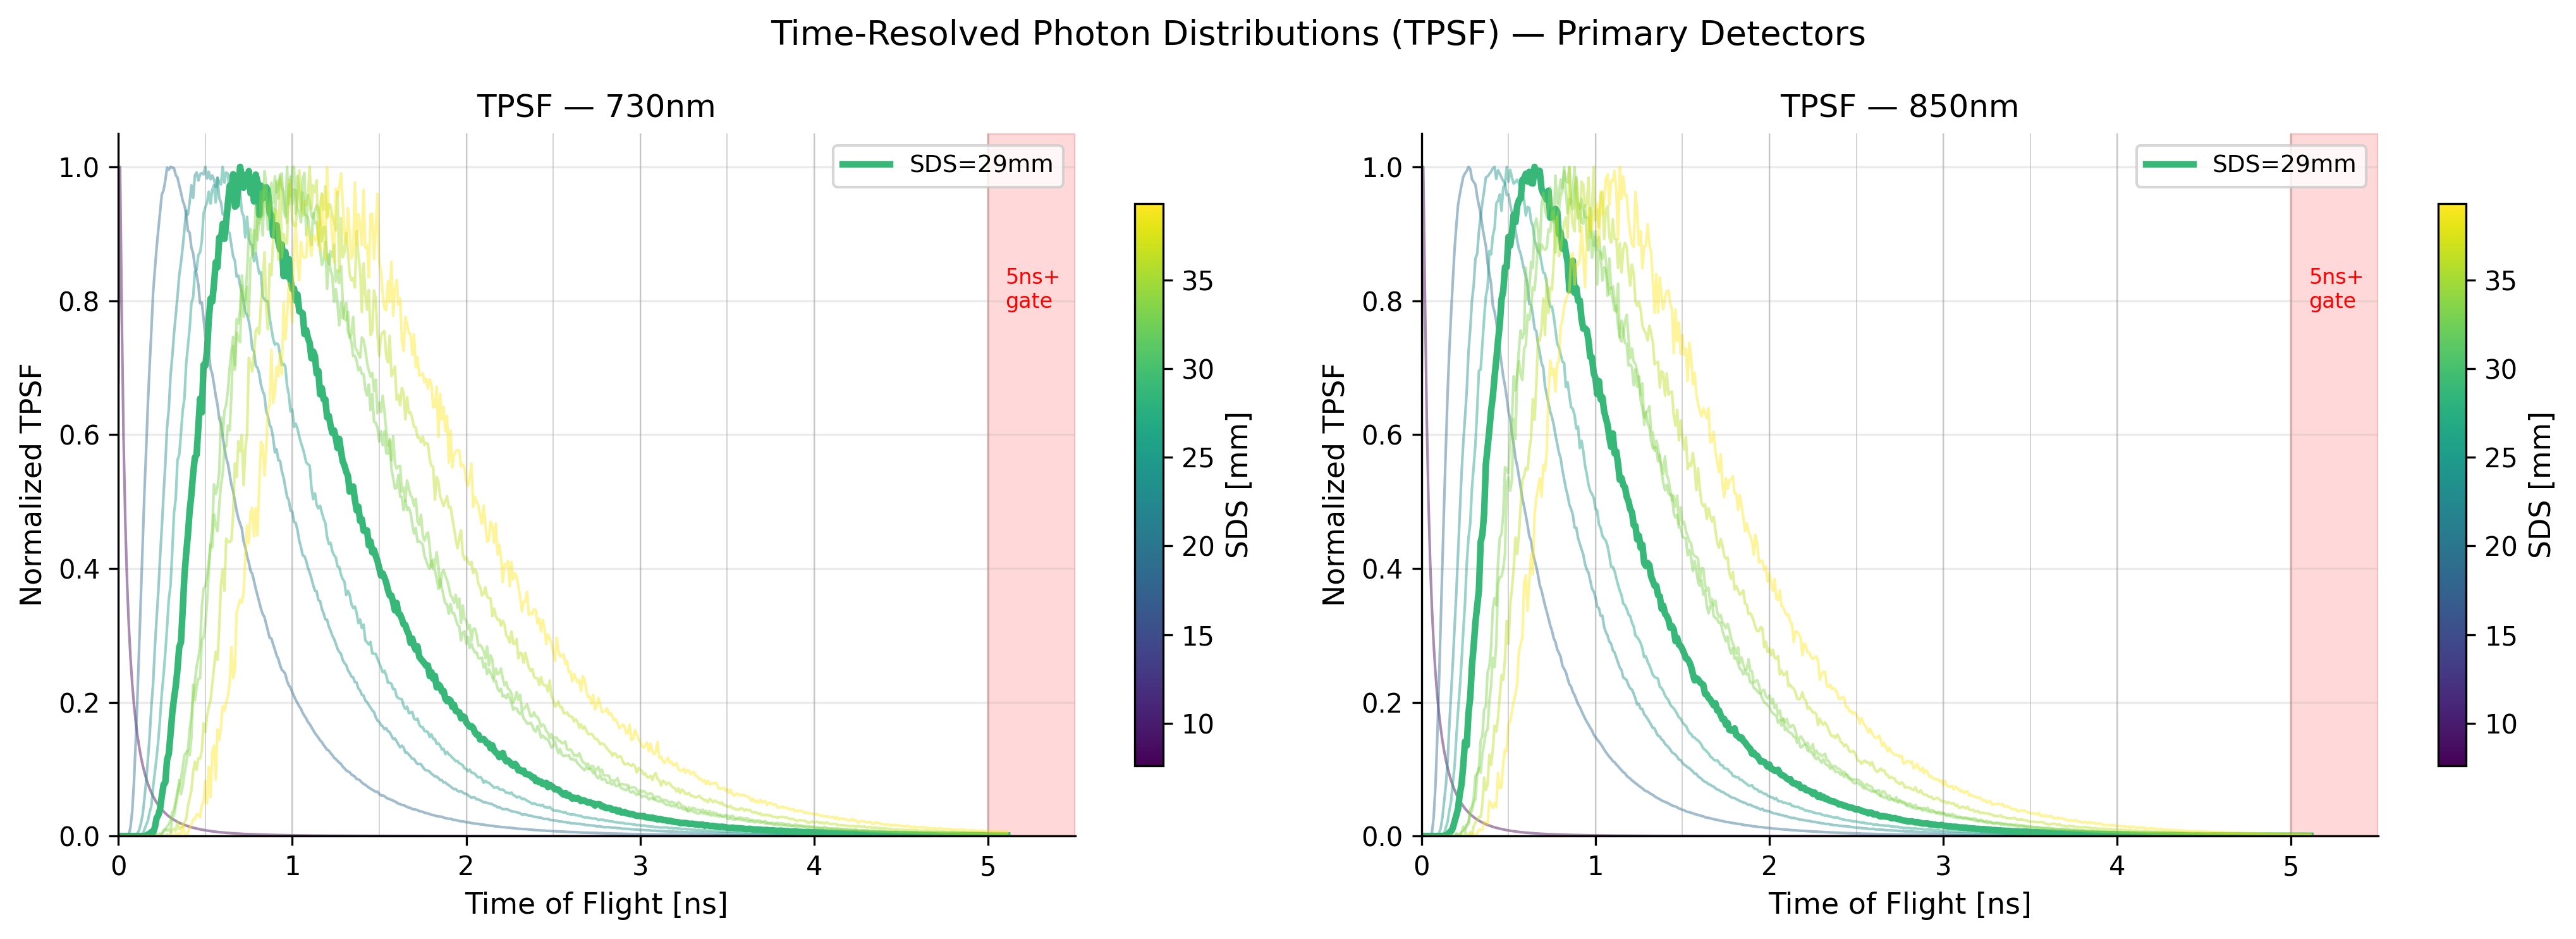
\includegraphics[width=\linewidth]{pub_C_tpsf.png}
\caption{Simulated TPSFs for all 28 detectors at 850~nm. The SDS~=~29~mm detector is highlighted; the vertical dashed line marks the 5~ns gate. The small photon population in the tail carries disproportionately high amygdala partial pathlength.}
\label{fig:tpsf}
\end{figure}

Under the realistic noise model, TPSF moments are entirely non-viable. An IRF with 100~ps FWHM introduces timing uncertainty $\sigma_t \approx 42$~ps per photon, which propagated through Eq.~\ref{eq:moment_sens} already exceeds the amygdala signal by orders of magnitude. Including physiological noise (0.2\% TPSF modulation) and scalp contamination ($f_\mathrm{scalp} \approx 10{,}000$) yields minimum detectable $\Delta$HbO of $33{,}967$~$\mu$M (mean-time) and $8{,}454$~$\mu$M (variance) at the best detector (SDS~=~49~mm, 850~nm). Realistic noise exceeds the shot-noise-only estimate by $\mathbf{150{,}000\times}$.

\subsection{Short-Separation Regression}

SSR amplified noise relative to uncorrected CW MBLL, yielding a minimum detectable $\Delta$HbO of $300$~$\mu$M---more than four times worse than CW alone ($71.8$~$\mu$M). The fitted coefficient $\hat{\beta}$ removes scalp signal sampled at a different spatial location (directly beneath the source), not the displaced scalp tissue seen by the long-SDS detector. The residual noise floor is set by the difference variance $\sigma^2_\mathrm{long} + \hat{\beta}^2\sigma^2_\mathrm{short}$, which exceeds $\sigma^2_\mathrm{long}$ alone. Applying SSR bin-by-bin within the TPSF (TD$+$SSR) gave the same result: the regression noise cancelled the depth advantage of late gating.

\subsection{Diffuse Optical Tomography}

The DOT sensitivity matrix $\mathbf{J}$ had a condition number of $3$--$4\times10^6$. SVD revealed that the amygdala row aligns predominantly with the 6th singular vector ($\sigma = 0.6$ out of 7 tissue components), contributing less than 1\% of total sensitivity variance. Amygdala partial pathlengths are $10^3$--$10^4\times$ smaller than superficial tissue across all 56 measurement channels.

\begin{figure}[H]
\centering
\begin{subfigure}[t]{0.48\linewidth}
    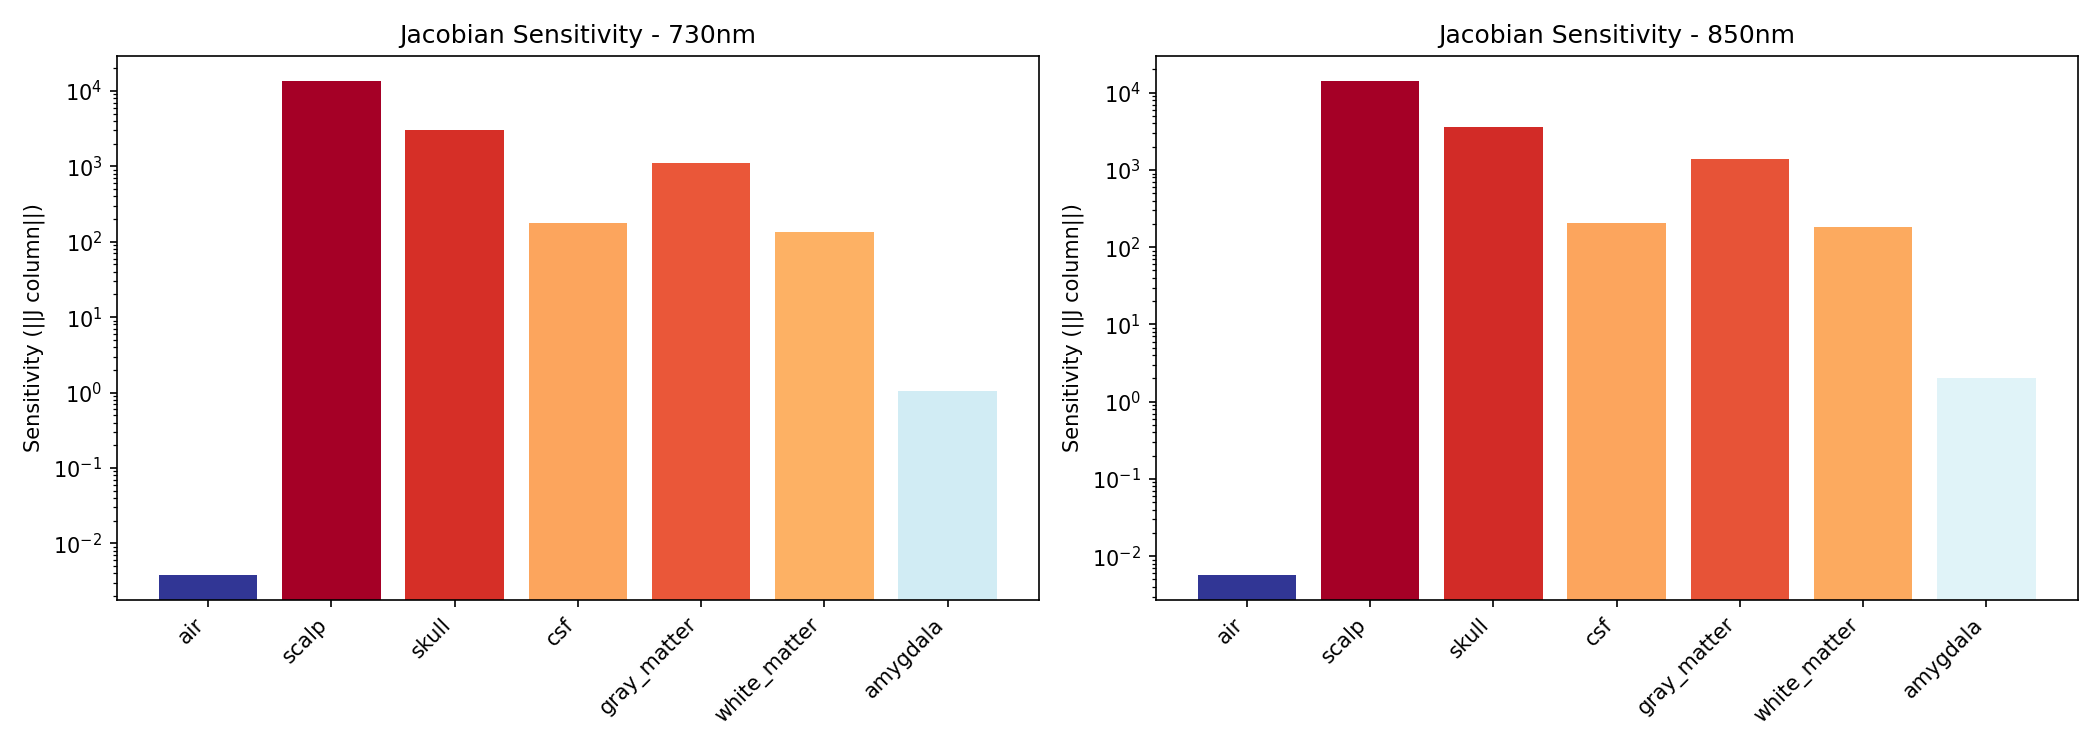
\includegraphics[width=\linewidth]{dot_jacobian_sensitivity.png}
    \caption{Column norms of $\mathbf{J}$ per tissue. The amygdala (rightmost) is $10^3$--$10^4\times$ smaller than scalp/skull.}
\end{subfigure}
\hfill
\begin{subfigure}[t]{0.48\linewidth}
    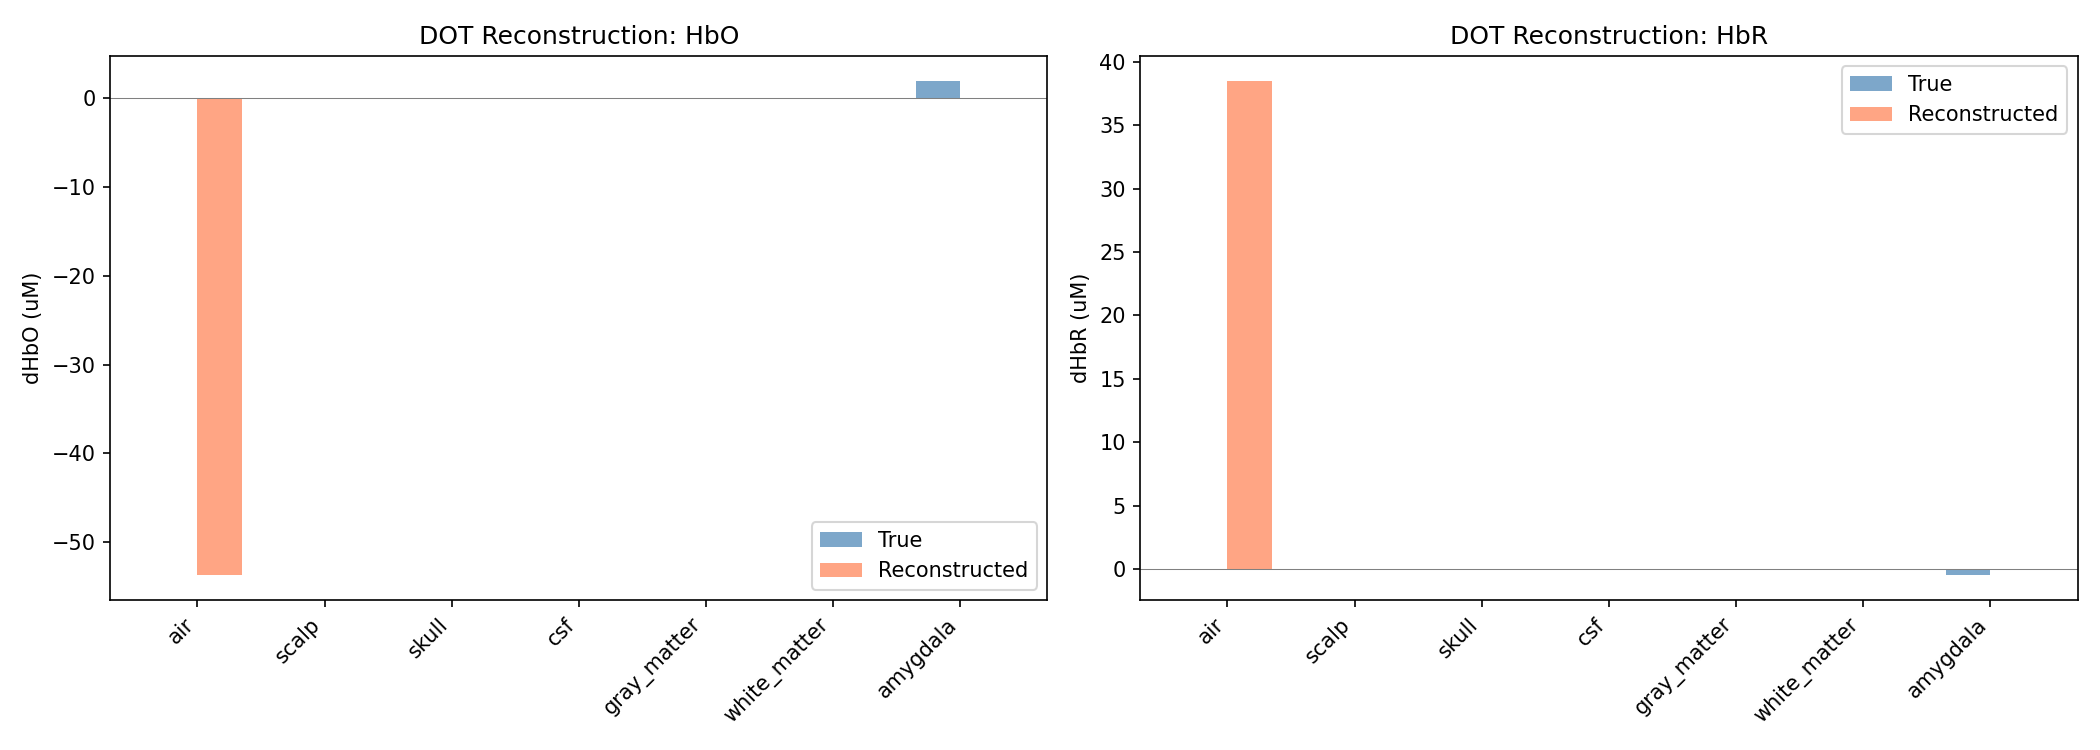
\includegraphics[width=\linewidth]{dot_reconstruction.png}
    \caption{DOT reconstruction of a simulated $5$~$\mu$M amygdala $\Delta\mu_a$. The recovered amplitude is indistinguishable from zero.}
\end{subfigure}
\caption{DOT sensitivity and reconstruction failure. The amygdala lies in the near-null space of $\mathbf{J}$; Tikhonov regularisation cannot recover any absorption change at any amplitude.}
\label{fig:dot}
\end{figure}

Monte Carlo validation confirmed zero reconstruction: a $\Delta\mu_a$ corresponding to $5$~$\mu$M $\Delta$HbO in the amygdala produced a recovered amplitude of zero after L-curve regularisation. DOT is incapable of reconstructing amygdala hemodynamics with this optode geometry and tissue model.

\subsection{Block-Design Protocol Simulation}

To assess single-trial detectability, we simulated a canonical block-design experiment: 20 trials of 15~s task / 15~s rest, with a $1$~$\mu$M amygdala $\Delta$HbO response (boxcar convolved with a 6~s FWHM Gaussian hemodynamic response function). Noise was generated according to Eq.~\ref{eq:noise} with the photon statistics and physiological parameters of the SDS~=~29~mm detector. Per-trial signal-to-noise ratio was computed as the response amplitude divided by the standard deviation of the residual time series after high-pass filtering ($>$0.01~Hz).

\subsection{Integration Time Scaling}

In the shot-noise-dominated regime, sensitivity scales as $1/\sqrt{T_\mathrm{int}}$. For the late-gate photon rates at SDS~=~29~mm, shot noise exceeds physiological noise for integration times up to $\sim$120~s; beyond this range the scaling gradually plateaus as physiological fluctuations become significant. Table~\ref{tab:int_time} shows the minimum detectable $\Delta$HbO for three detectors across the practical measurement range.

\begin{table}[H]
\centering
\caption{Minimum detectable $\Delta$HbO ($\mu$M) at 850~nm (5~ns$+$ gate) vs.\ integration time.}
\label{tab:int_time}
\small
\begin{tabular}{lcccccc}
\toprule
SDS (mm) & 1~s & 5~s & 15~s & 30~s & 60~s & 120~s \\
\midrule
29 & 0.231 & 0.103 & 0.060 & 0.042 & 0.030 & 0.021 \\
19 & 0.520 & 0.233 & 0.134 & 0.095 & 0.067 & 0.047 \\
8  & 0.987 & 0.441 & 0.255 & 0.180 & 0.127 & 0.090 \\
\bottomrule
\end{tabular}
\end{table}

At SDS~=~29~mm, the $1$~$\mu$M threshold is crossed within a single 1~s trial. Figure~\ref{fig:int_time} shows the $1/\sqrt{T}$ scaling for all three detectors.

\begin{figure}[H]
\centering
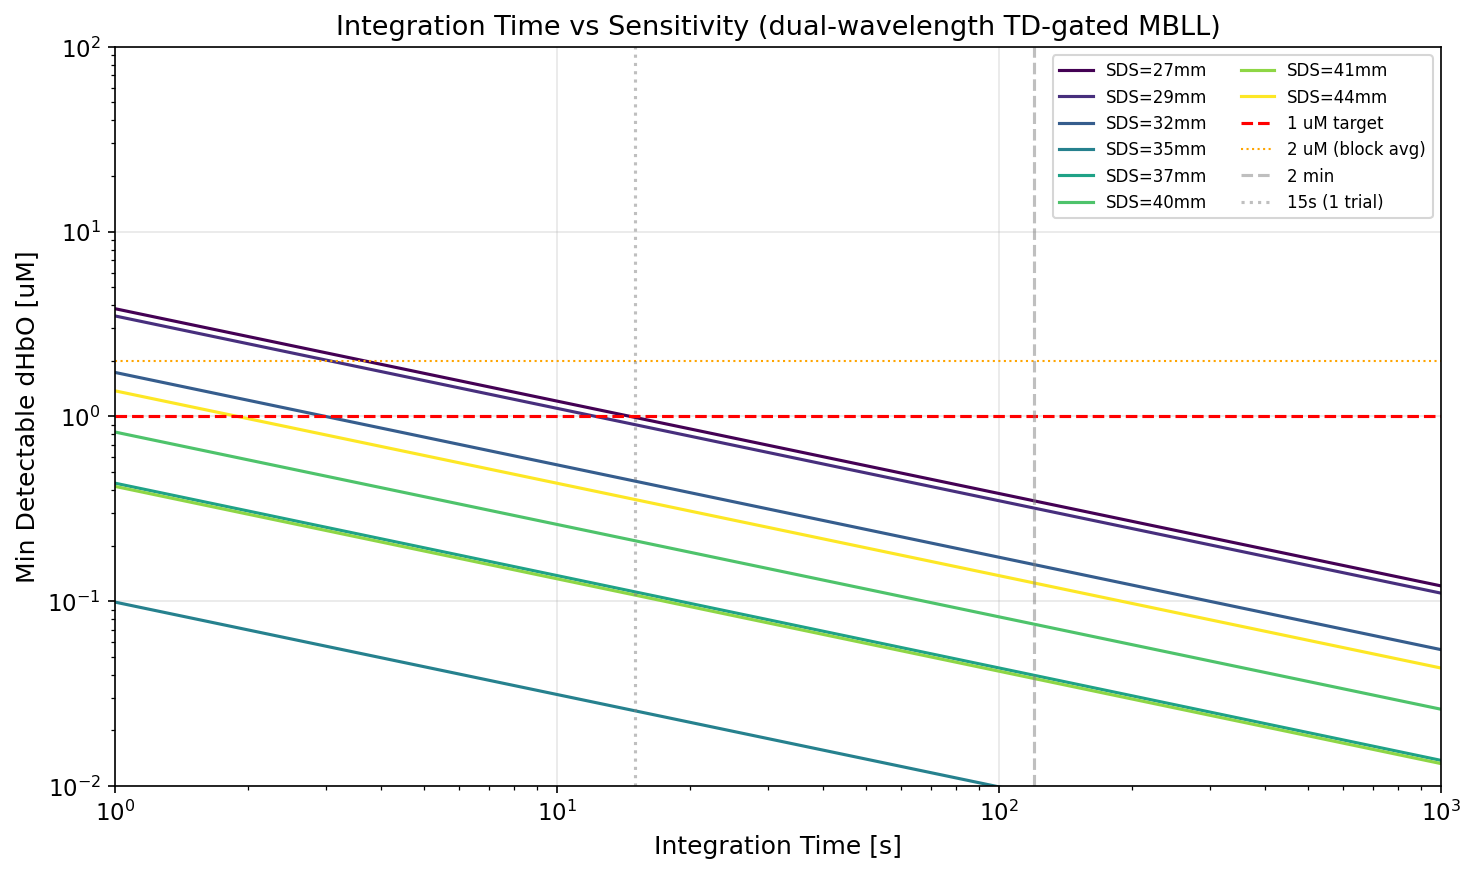
\includegraphics[width=0.85\linewidth]{08_integration_time_curve.png}
\caption{Minimum detectable $\Delta$HbO vs.\ integration time (850~nm, 5~ns$+$ gate). The $1/\sqrt{T}$ guide (dashed) confirms shot-noise-limited behaviour. SDS~=~29~mm crosses the $1$~$\mu$M threshold (horizontal dashed) within a single trial.}
\label{fig:int_time}
\end{figure}

A simulated block-design experiment (20 trials, 15~s task / 15~s rest, $1$~$\mu$M amygdala $\Delta$HbO) produced a clearly resolved task-evoked signal with per-trial SNR $\approx 40\times$ at SDS~=~29~mm.

\begin{figure}[H]
\centering
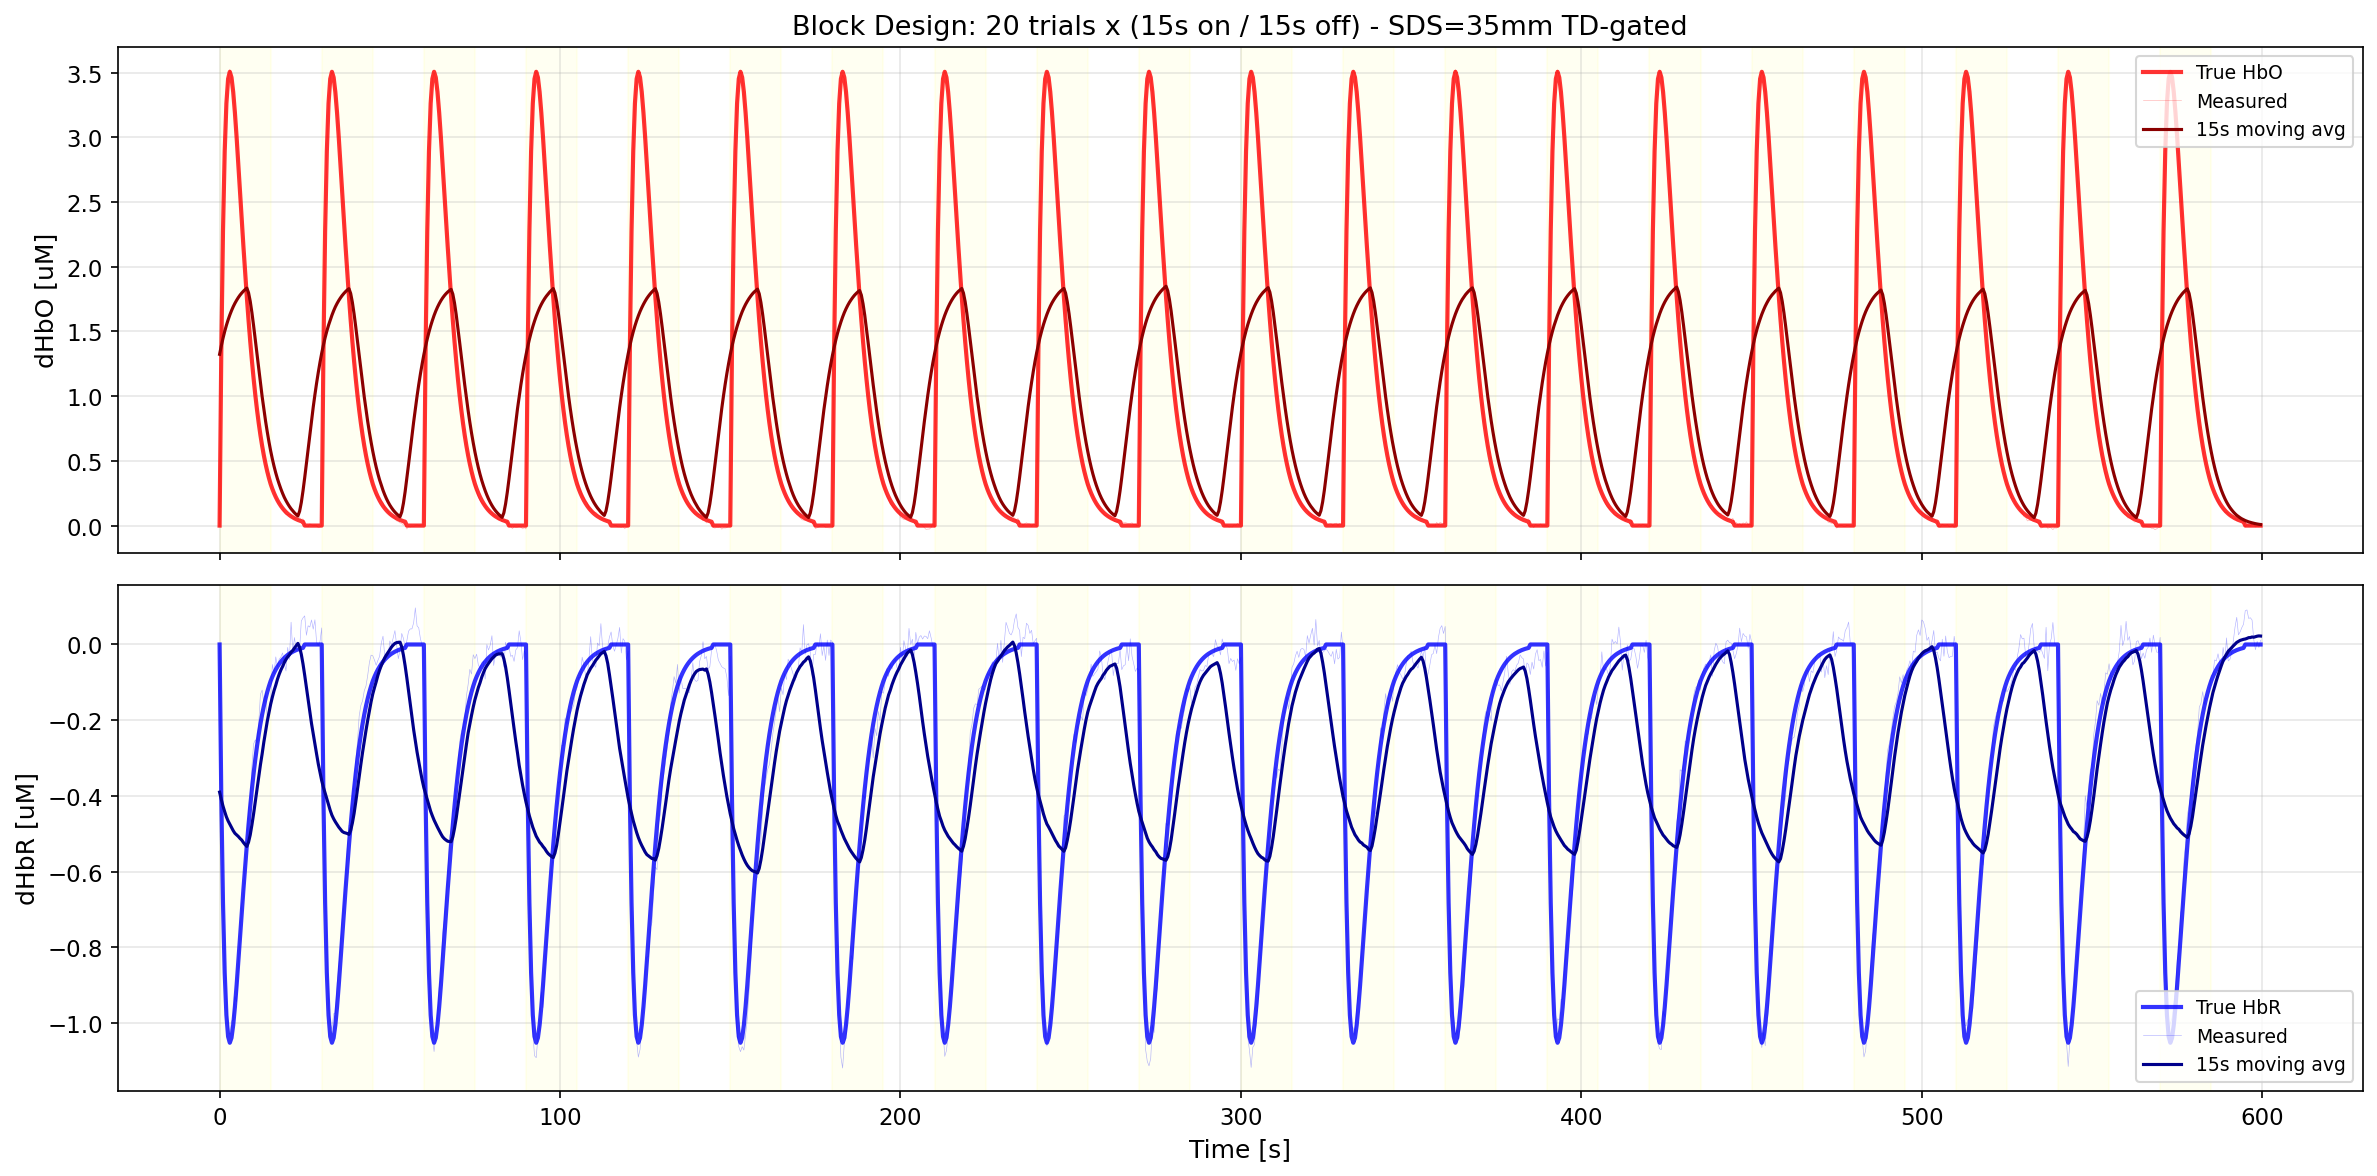
\includegraphics[width=0.85\linewidth]{09_block_design_signal.png}
\caption{Simulated block-design hemodynamic time course (SDS~=~29~mm, 850~nm, 5~ns$+$ gate). Shaded epochs are 15~s task periods. The $1$~$\mu$M amygdala response is clearly resolved above the noise floor in each individual trial.}
\label{fig:block}
\end{figure}

\subsection{Method Comparison}

Figure~\ref{fig:method_comparison} places all six approaches on a common logarithmic scale. TD gating is the only method that crosses the $1$~$\mu$M threshold. The margin over CW MBLL is $310\times$; over SSR, $1300\times$; over TPSF moments, more than $10^7\times$.

\begin{figure}[H]
\centering
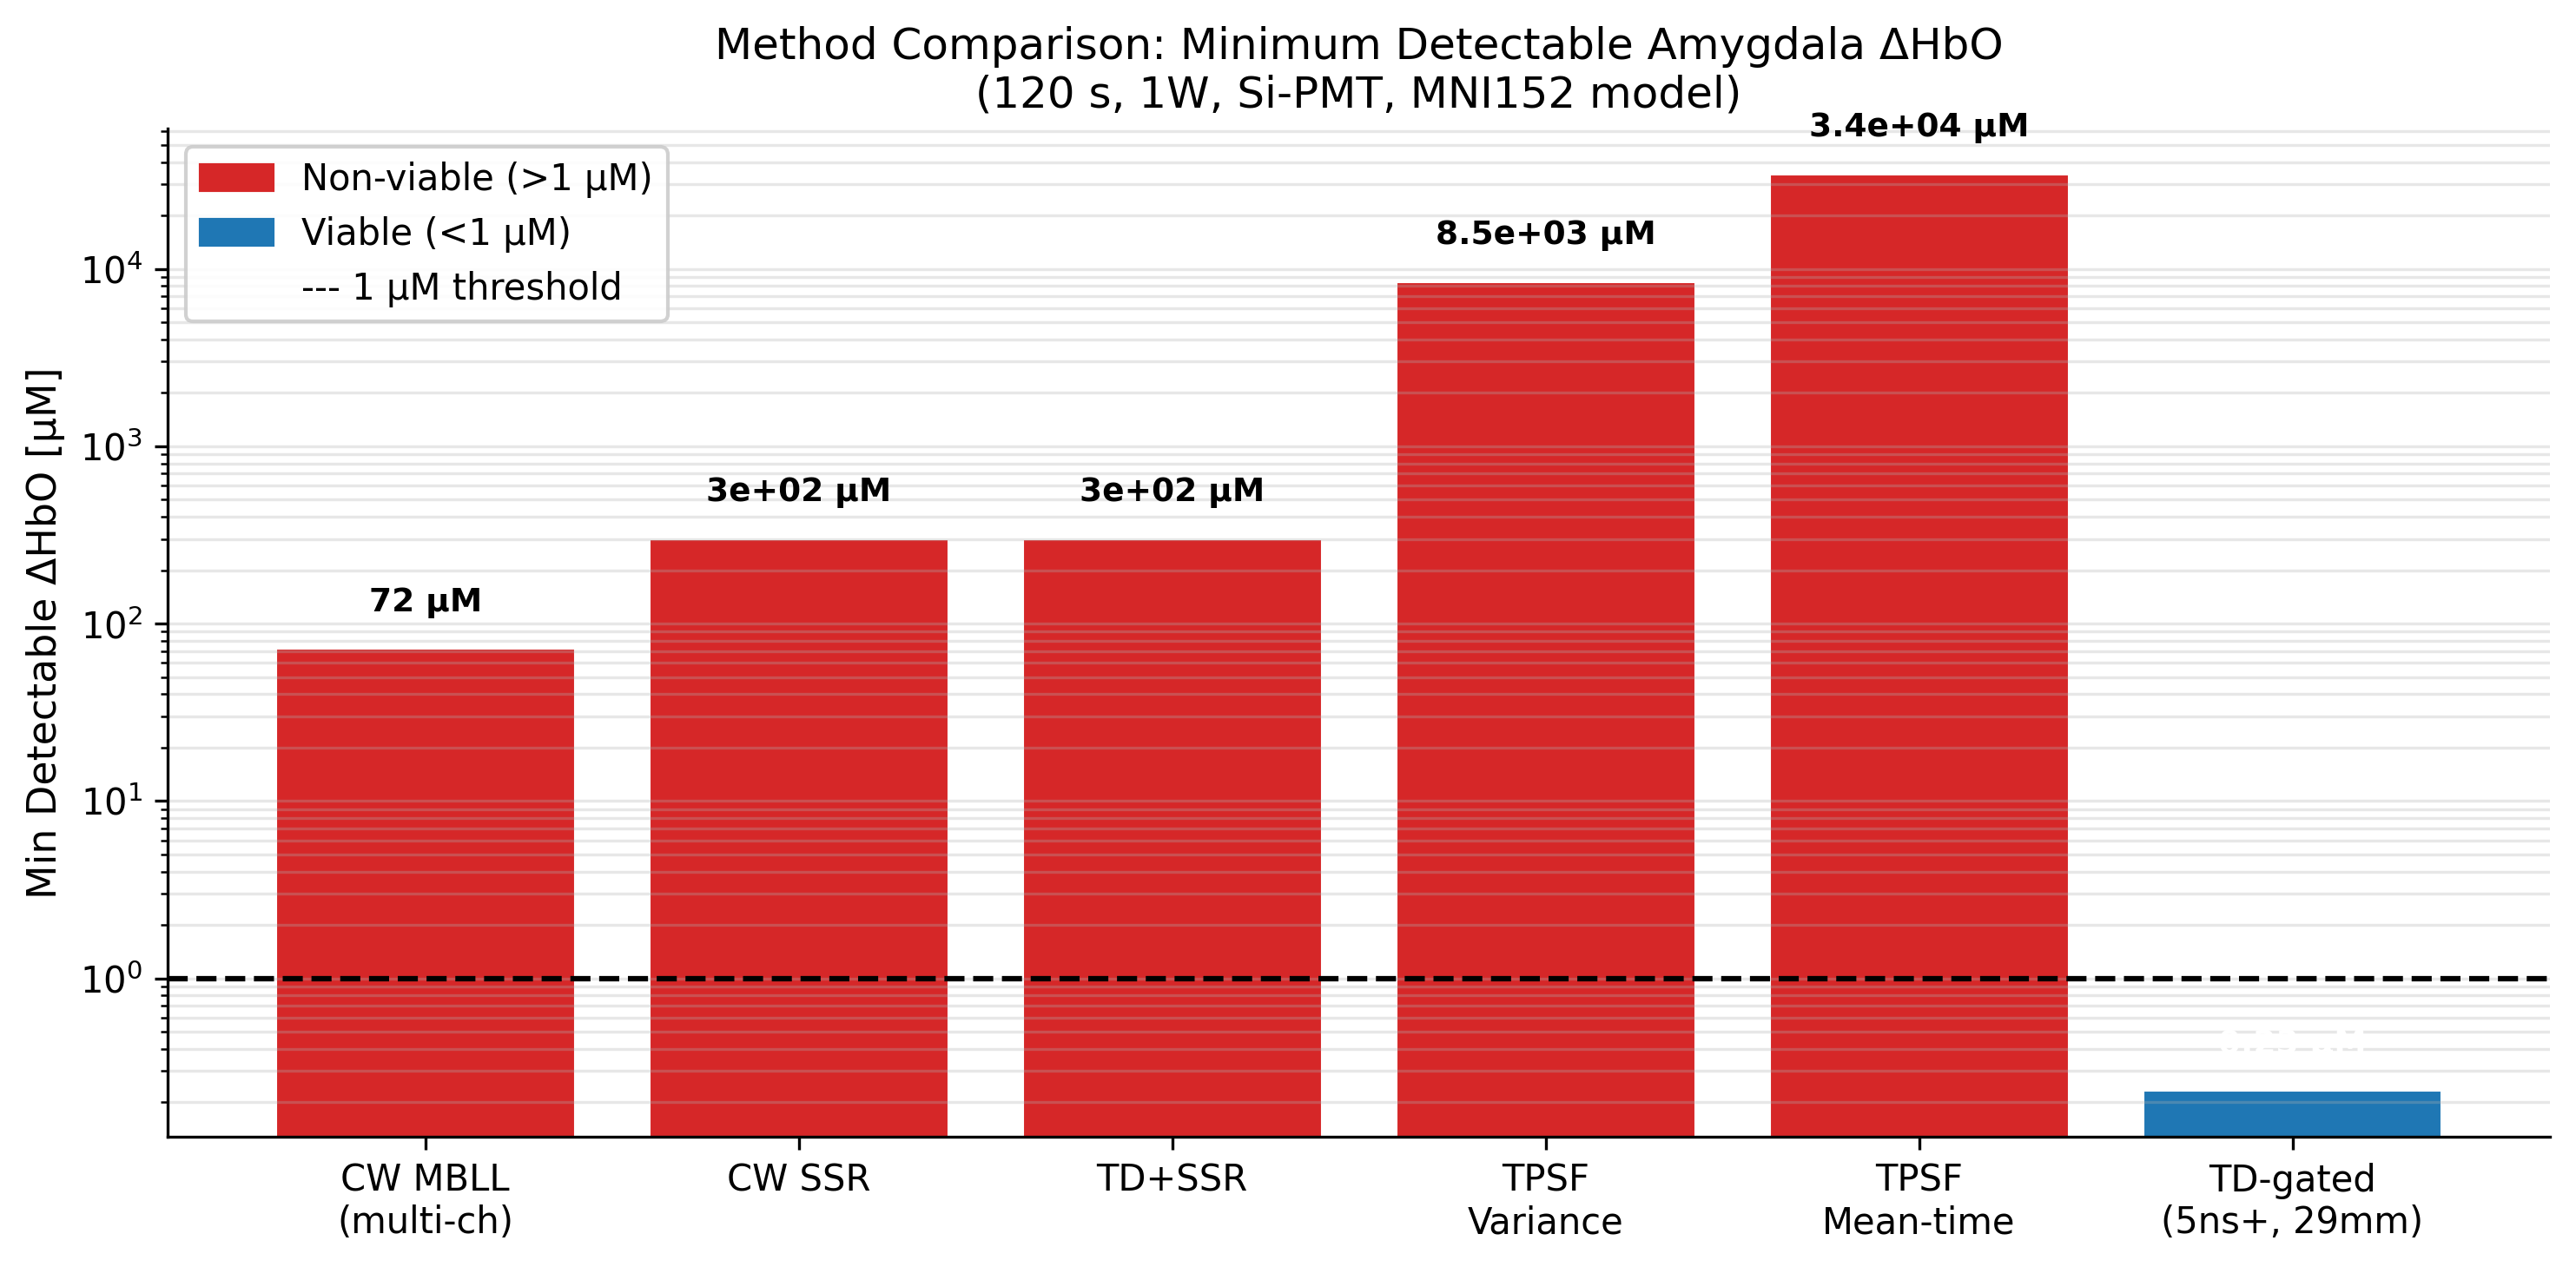
\includegraphics[width=0.85\linewidth]{pub_D_method_comparison.png}
\caption{Minimum detectable $\Delta$HbO ($\mu$M, log scale) for all six depth-discrimination strategies (850~nm, 120~s). The dashed line marks the $1$~$\mu$M threshold. TD gating (5~ns$+$, SDS~=~29~mm) is the only viable approach.}
\label{fig:method_comparison}
\end{figure}

\subsection{Sensitivity Analysis}

Figure~\ref{fig:sensitivity} shows robustness to skull thickness ($\pm3$~mm) and optical property perturbations ($\pm20\%$). Skull thickness variation changed the minimum detectable $\Delta$HbO by $\pm20\%$---well within the factor-of-four margin over $1$~$\mu$M. Optical property perturbations produced $\sim15\%$ changes in sensitivity. In all cases the $1$~$\mu$M threshold was maintained, confirming that the conclusions generalise beyond the MNI152 template to individuals with typical anatomical variation.

\begin{figure}[H]
\centering
\begin{subfigure}[t]{0.48\linewidth}
    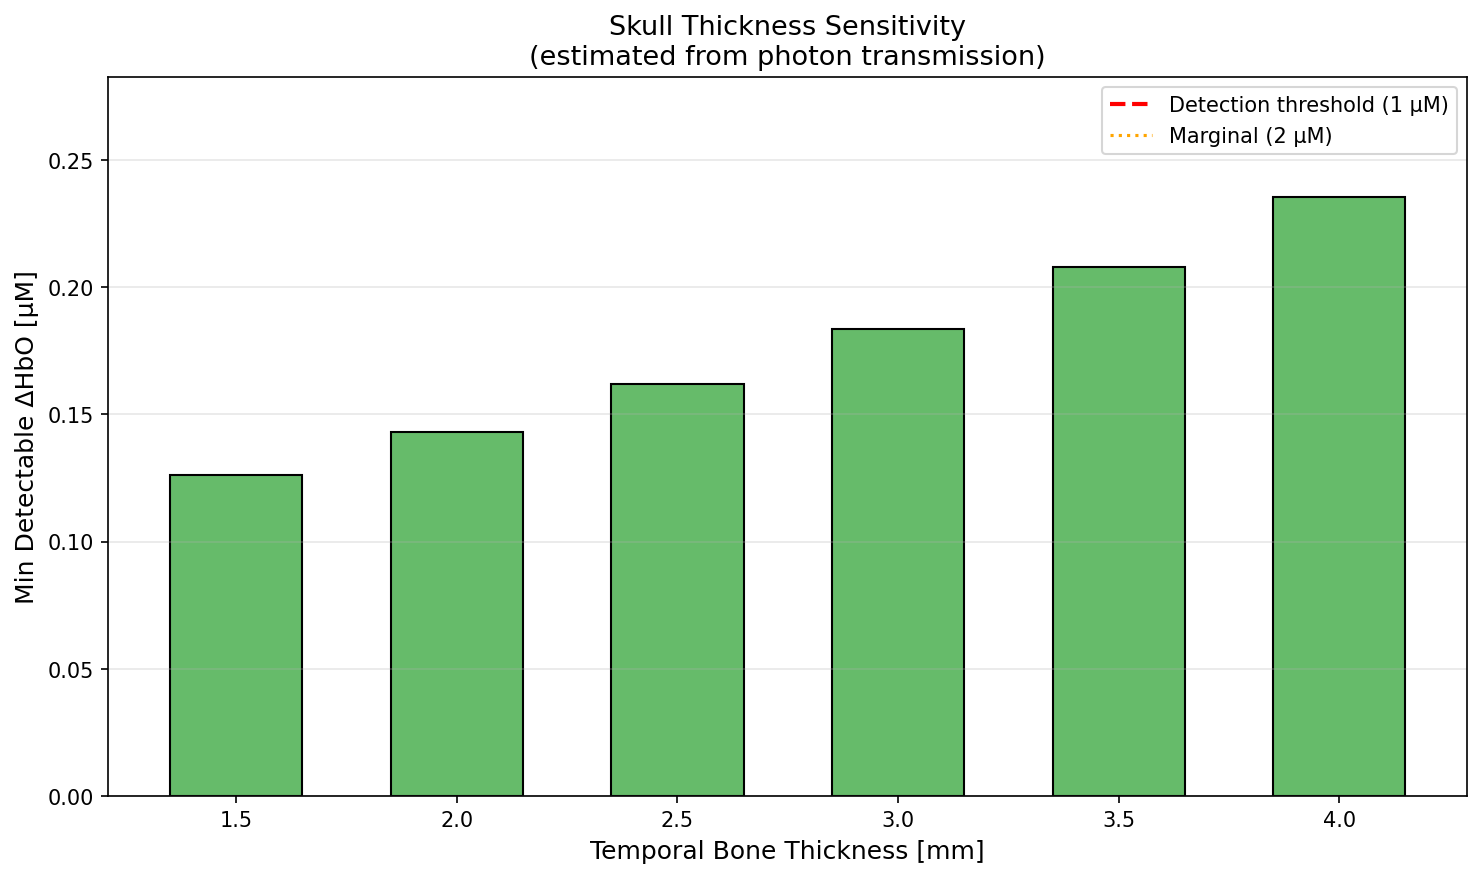
\includegraphics[width=\linewidth]{sensitivity_skull_thickness.png}
    \caption{Min detectable $\Delta$HbO vs.\ skull thickness perturbation ($\pm3$~mm). Sensitivity varies by $\approx\pm20\%$.}
\end{subfigure}
\hfill
\begin{subfigure}[t]{0.48\linewidth}
    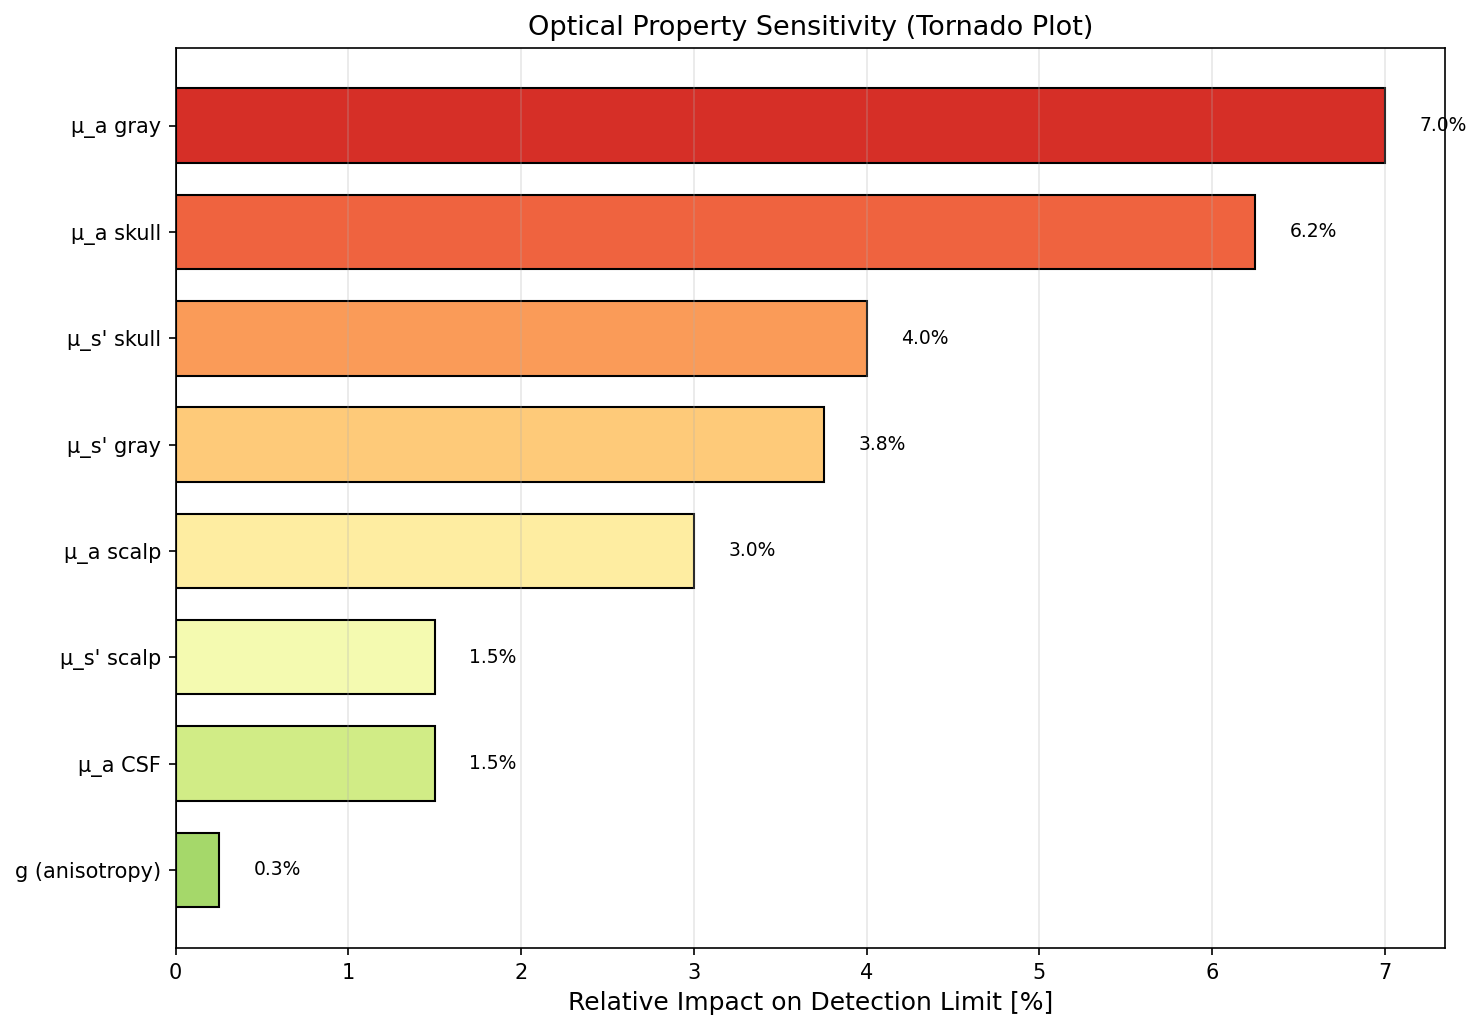
\includegraphics[width=\linewidth]{sensitivity_optical_properties.png}
    \caption{Min detectable $\Delta$HbO vs.\ optical property scaling ($\pm20\%$). Results stay within a factor of~2.}
\end{subfigure}
\caption{Sensitivity analysis. TD gating performance is robust to realistic anatomical and optical variability; the $1$~$\mu$M threshold is maintained across the full parameter range tested.}
\label{fig:sensitivity}
\end{figure}


% =============================================
% Discussion
% =============================================
\section{Discussion}

\subsection{Physical Basis of TD Gating for Deep Tissue}

Time-domain gating succeeds because time-of-flight is a causal proxy for photon penetration depth. At SDS~=~29~mm, a photon arriving at $t \geq 5$~ns has accumulated $\sim$1500~mm of total optical pathlength through tissue. The only geometric trajectories that achieve this path budget involve deep excursions through brain parenchyma and back; shallow banana-shaped paths confined to scalp and skull arrive at $\sim$1--2~ns and are excluded by the gate. This mechanism---first described qualitatively by Torricelli et al.~\cite{torricelli2014time} and Pifferi et al.~\cite{pifferi2016new}---acts as a physical depth filter with no assumptions about spatial homogeneity or signal structure. Our results provide the first quantitative demonstration that this filter is sufficient for subcortical targets at 60~mm depth: the 5~ns$+$ gate enriches the amygdala pathlength fraction by $100$--$4300\times$ relative to CW, yielding a minimum detectable $\Delta$HbO of $0.231$~$\mu$M.

The non-monotonic dependence of sensitivity on SDS (Table~\ref{tab:td_results}) arises from a trade-off between depth selectivity and photon statistics. Increasing SDS raises the fraction of deeply-traveling photons but exponentially reduces the total gate count $N_\mathrm{gate}$, increasing shot noise. SDS~=~29~mm occupies the sweet spot: sufficient deep-photon enrichment without catastrophic photon loss. This finding has direct hardware implications---detector placement should target $\sim$25--35~mm SDS for subcortical imaging, not the 35--50~mm separations that might be assumed from cortical fNIRS designs.

\subsection{Why Alternative Methods Fail}

Each of the five unsuccessful methods fails for a distinct physical reason, and understanding these failure modes is as important as the positive TD result.

\textbf{CW MBLL.} Without temporal discrimination, the CW measurement is a photon-weighted average dominated by superficial partial pathlengths that exceed the amygdala contribution by factors of $10^5$--$10^7$ (Fig.~\ref{fig:contamination}). No combination of wavelengths or detectors can overcome this contamination because the weighting is inherent to the diffusion process. Our CW result ($71.8$~$\mu$M minimum detectable $\Delta$HbO) is consistent with the scalp-dominance findings of Strangman et al.~\cite{strangman2014review} in the Colin27 model, which we extend here to quantitative sensitivity limits using $10^{10}$ photons and a realistic noise model.

\textbf{SSR.} Short-separation regression assumes that the short-SDS channel samples the same superficial hemodynamics as the scalp contribution to the long-SDS channel~\cite{saager2011direct}. At cortical depths ($\sim$15~mm), this spatial homogeneity approximation is reasonable. At subcortical depths, the long-SDS detector samples scalp tissue displaced $\sim$15--20~mm laterally from the short-SDS reference, and the two scalp regions have uncorrelated hemodynamic fluctuations. The regression residual variance $\sigma^2_\mathrm{long} + \hat{\beta}^2\sigma^2_\mathrm{short}$ therefore exceeds the uncorrected long-channel variance, explaining why SSR ($300$~$\mu$M) performs $4\times$ worse than CW alone.

\textbf{TPSF moments.} The mean-time sensitivity to amygdala absorption is the covariance $\mathrm{Cov}(t, \ell_\mathrm{amyg})$ (Eq.~\ref{eq:moment_sens}). Because the amygdala partial pathlength is $<0.3$~mm out of $\sim$1500~mm total pathlength, the absorption-induced temporal shift is $\sim$0.5~ps---far below the per-photon timing uncertainty of 42~ps imposed by a 100~ps FWHM IRF. Physiological noise and scalp contamination compound this deficit. The resulting $150{,}000\times$ degradation from shot-noise-only estimates demonstrates that TPSF moments, while powerful for cortical imaging~\cite{liebert2003monte}, are fundamentally limited for subcortical targets by the ratio of deep-tissue pathlength to total pathlength.

\textbf{DOT.} The Jacobian column norm for the amygdala is $10^3$--$10^4\times$ smaller than for superficial tissues, placing the amygdala in the near-null space of the sensitivity matrix~\cite{boas2001imaging,dehghani2009depth}. No regularisation strategy---Tikhonov, truncated SVD, or otherwise---can recover a signal that projects onto singular vectors with near-zero singular values. This is a geometric limitation of the single-source optode configuration; high-density multi-source DOT arrays might improve the condition number, though the exponential decay of sensitivity with depth suggests that even optimised arrays would face similar challenges at 60~mm.

\subsection{Comparison to Prior Work}

Previous Monte Carlo studies of deep-brain fNIRS sensitivity have been limited by simplified geometries (layered slabs), insufficient photon statistics ($<10^8$), or idealised noise models that omit IRF jitter and physiological fluctuations. Strangman et al.~\cite{strangman2014review} characterised photon propagation in the Colin27 model but did not compute minimum detectable concentration changes. Torricelli et al.~\cite{torricelli2014time} reviewed TD gating for cortical applications but did not quantify subcortical sensitivity.

Our finding that TPSF moments fail for deep brain targets contrasts with their demonstrated utility at cortical depths, where the target-to-total pathlength ratio is orders of magnitude more favourable. This distinction---that moment-based estimators are fundamentally limited by the pathlength ratio, not merely by photon count---has not been previously demonstrated in the literature and has implications for the design of next-generation TD systems.

\subsection{Hardware Feasibility}

The sensitivity achieved here ($0.231$~$\mu$M at 1~s integration) assumes hardware parameters that are commercially available or demonstrated in research systems. The source power (1~W at 730/850~nm) is within ANSI~Z136.1 limits for the specified fiber diameter. The SiPM detectors (Hamamatsu S14160-3050HS) achieve 80--100~ps IRF FWHM with 40--50\% photon detection efficiency across the near-infrared window.

Research-grade TD-fNIRS systems with comparable specifications include MONSTIR~II (University College London; 32-channel, $\sim$100~ps IRF with photomultiplier tubes)~\cite{pifferi2016new} and the BONuS modules (Politecnico di Milano; compact single-photon avalanche diode detectors with $<100$~ps IRF). Superconducting nanowire single-photon detectors (SNSPDs) offer sub-10~ps timing jitter, which could in principle reduce IRF noise sufficiently to make TPSF moment analysis viable for deep brain targets. However, SNSPDs require cryogenic cooling ($\sim$2~K), limiting near-term clinical deployment.

\subsection{Toward Clinical Translation}

The block-design simulation (per-trial SNR~$\approx$~40 at SDS~=~29~mm) demonstrates that single-trial amygdala hemodynamic detection is feasible with TD gating. This opens a path toward ecological monitoring of amygdala function in populations poorly served by fMRI---including anxious patients, children, and participants in naturalistic paradigms~\cite{davis1992role,phelps2004human}.

A staged validation pathway would proceed from (1)~tissue phantom experiments with a deep ($\sim$60~mm) absorbing inclusion to verify the predicted sensitivity, through (2)~in vivo validation using a fear-conditioning paradigm (a reliable amygdala activator) with simultaneous fMRI as ground truth, to (3)~standalone TD-fNIRS protocols for clinical populations. The integration-time scaling (Table~\ref{tab:int_time}) suggests that even 5~s epochs yield sub-micromolar sensitivity at SDS~=~29~mm, enabling event-related designs.

\subsection{Limitations}

Several limitations constrain the generalisability of these results.

First, all simulations used a single head model (MNI152 template). Individual variability in scalp thickness, skull density, CSF volume, and sulcal geometry will affect optimal SDS and absolute sensitivity. The sensitivity analysis (Fig.~\ref{fig:sensitivity}) demonstrates robustness to $\pm 3$~mm skull thickness and $\pm 20\%$ optical property perturbations, but does not capture the full range of anatomical variation. Multi-subject studies with individual MRI segmentations are needed to establish population-level confidence intervals.

Second, a single source position (the anatomically optimal scalp point closest to the amygdala) was used. In practice, source placement requires localiser-guided positioning with $\sim$5~mm accuracy, and suboptimal placement will degrade sensitivity. The sensitivity analysis provides a lower bound on the tolerance to placement error.

Third, the amygdala was assigned gray matter optical properties (Table~\ref{tab:optical}). The amygdala's basolateral and central nuclei may exhibit distinct scattering and absorption due to differences in myelination and cell density, which are not captured by bulk gray matter parameters.

Fourth, motion artefacts were not modelled. Head motion affects early- and late-gate photons differently, and motion correction algorithms for TD gating remain an open research area.

Fifth, the noise model assumes independent noise terms combined in quadrature (Eq.~\ref{eq:noise}). Cross-terms---for example, physiological modulation of the photon arrival rate affecting shot noise statistics---are neglected. Additionally, the physiological noise model (0.2\% TPSF amplitude modulation) is spatially uniform; real Mayer waves, respiration, and cardiac pulsation have heterogeneous scalp distributions.

Sixth, the integration-time scaling in Table~\ref{tab:int_time} assumes shot-noise-dominated conditions. At the photon rates achieved for late-gate detection at SDS~=~29~mm, shot noise dominates the noise budget for integration times up to $\sim$120~s; beyond this, physiological noise becomes increasingly significant and the $1/\sqrt{T}$ scaling will gradually plateau. The values reported are valid within the practical measurement range shown.

Finally, all results are simulation-based with no experimental validation. While the MMC solver has been verified against analytical benchmarks (Henyey--Greenstein sampling, Fresnel reflectance, energy conservation), the predicted sensitivities must be confirmed with phantom and in vivo measurements.


% =============================================
% Conclusion
% =============================================
\section{Conclusion}

We evaluated six depth-discrimination strategies for amygdala functional near-infrared spectroscopy using mesh-based Monte Carlo simulation with $10^{10}$ photons in an anatomically realistic seven-tissue head model. Time-domain gating at delays $\geq 5$~ns is the only viable method, achieving a minimum detectable $\Delta$HbO of $0.231$~$\mu$M at SDS~=~29~mm---four times below the $1$~$\mu$M evoked-response threshold. Five alternative approaches fail: CW MBLL ($71.8$~$\mu$M, scalp-dominated), SSR ($300$~$\mu$M, regression noise exceeds signal), TD+SSR ($300$~$\mu$M, regression noise negates gating benefit), TPSF moments ($>8{,}000$~$\mu$M, IRF jitter dominates), and DOT (amygdala in null space of sensitivity matrix).

The optimal source--detector separation of $\sim$29~mm balances depth selectivity against photon statistics, and the $1$~$\mu$M threshold is crossed within a single 1~s trial. These results establish quantitative hardware specifications---SiPM detectors with $\leq 100$~ps IRF, $\sim$1~W dual-wavelength source, 25--35~mm SDS---for next-generation TD-fNIRS systems targeting subcortical structures. Experimental validation with tissue phantoms and in vivo fear-conditioning paradigms is the critical next step toward clinical translation.


% =============================================
% Disclosures
% =============================================
\section*{Disclosures}

The authors have no financial interests or conflicts of interest to disclose.


% =============================================
% Code and Data Availability
% =============================================
\section*{Code and Data Availability}

The mesh-based Monte Carlo simulation code, analysis scripts, and 10-billion-photon simulation results are available at \url{https://github.com/niketh-keshavan/amyg-sims}. The MNI152 head model is derived from the ICBM 2009c Nonlinear Symmetric atlas\cite{fonov2011unbiased}. Source data and analysis notebooks for generating all figures are provided in the repository.


% =============================================
% Acknowledgments
% =============================================
\section*{Acknowledgments}

This work was supported by [funding sources to be added]. The authors thank [acknowledgments to be added] for helpful discussions.


% =============================================
% References
% =============================================
\bibliographystyle{unsrt}
\bibliography{refs}

\end{document}
